\documentclass[12pt,a4paper,twoside]{report}

% ======================
% Packages
% ======================
\usepackage[utf8]{inputenc}
\usepackage[T1]{fontenc}
\usepackage[french]{babel}
\usepackage{times}
\usepackage{geometry}
\geometry{margin=2.5cm}
\usepackage{setspace}
\setstretch{1.15}

\usepackage{graphicx}
\usepackage{caption}
\usepackage{float}
\usepackage{fancyhdr}
\usepackage{titlesec}
\usepackage{ragged2e}
\usepackage{tcolorbox}
\usepackage{hyperref}
\usepackage{lastpage}
\usepackage{xcolor}
\usepackage{booktabs}
\usepackage{array}
\usepackage{longtable}
\usepackage{enumitem}
\usepackage{amsmath}
\usepackage{listings}
\usepackage{tikz}
\usetikzlibrary{shapes.geometric, arrows, arrows.meta, positioning, calc, backgrounds, fit, decorations.pathreplacing, shadings}
\definecolor{pwcorange}{RGB}{208,74,2}
\definecolor{pwcblack}{RGB}{29,29,27}
\definecolor{pwcgray}{RGB}{100,100,100}
\definecolor{deloitte}{RGB}{134,188,37}
\definecolor{ey}{RGB}{255,230,0}
\definecolor{kpmg}{RGB}{0,49,141}
\definecolor{crisppink}{RGB}{220,50,120}
\definecolor{crispamber}{RGB}{255,165,0}

% ======================
% Pagination
% ======================
\pagestyle{fancy}
\fancyhf{}
\fancyhead[LE,RO]{\nouppercase{\leftmark}}
\fancyfoot[R]{\thepage/\pageref{LastPage}}
\renewcommand{\headrulewidth}{0.4pt}

% ======================
% Paragraphes
% ======================
\setlength{\parindent}{0.5cm}
\justifying

% ======================
% Titres
% ======================
\titleformat{\chapter}[hang]{\bfseries\fontsize{16}{18}\selectfont}{\thechapter}{0.2cm}{}
\titlespacing*{\chapter}{0pt}{12pt}{12pt}
\titleformat{\section}[hang]{\bfseries\fontsize{14}{16}\selectfont}{\thesection}{0.2cm}{}
\titlespacing*{\section}{0pt}{10pt}{6pt}
\titleformat{\subsection}[hang]{\bfseries\fontsize{12}{14}\selectfont}{\thesubsection}{0.2cm}{}
\titlespacing*{\subsection}{0pt}{8pt}{4pt}

% ======================
% Définition encadrée
% ======================
\newtcolorbox{definitionbox}{
  colframe=black,
  colback=gray!5,
  boxrule=0.6pt,
  arc=2pt
}

% ======================
% Métadonnées
% ======================
\hypersetup{
  colorlinks=true,
  linkcolor=black,
  urlcolor=blue,
  citecolor=black,
  pdftitle={Détection intelligente d'anomalies financières},
  pdfauthor={Yousra Chaieb},
  pdfsubject={Projet de Fin d'Études --- Méthodologie CRISP-DM}
}

% ======================
% Listings (code)
% ======================
\lstset{
  basicstyle=\ttfamily\small,
  breaklines=true,
  frame=single,
  captionpos=b,
  numbers=left,
  numberstyle=\tiny,
  xleftmargin=1.5em
}

\begin{document}

\pagenumbering{gobble}

% =====================================================
% PAGE DE GARDE
% =====================================================
\begin{titlepage}
\centering

\vspace{1cm}

{\large \textbf{École Supérieure Privée d'Ingénierie et de Technologies --- ESPRIT}}\\[0.3cm]
{\large Département Informatique --- Filière Data Science \& IA}

\vspace{1.5cm}

\rule{\linewidth}{0.4pt}\\[0.4cm]
{\fontsize{24}{28}\selectfont \textbf{Détection intelligente\\[0.2cm] d'anomalies financières}}\\[0.4cm]
\rule{\linewidth}{0.4pt}

\vspace{0.6cm}

{\large \textit{Analyse de transactions, modélisation par apprentissage automatique\\et génération d'explications par modèle de langage}}

\vspace{1.5cm}

{\large Rapport de Projet de Fin d'Études}\\[0.2cm]
{\normalsize Réalisé dans le cadre du cycle ingénieur --- Spécialité Intelligence Artificielle}

\vspace{1.5cm}

\begin{tabular}{rl}
  \textbf{Réalisé par :}         & Yousra Chaieb \\[0.2cm]
  \textbf{Encadrant académique :} & Pr. Mohamed Islem Samaali \\[0.2cm]
  \textbf{Encadrants entreprise :} & Mr. Slim Zribi \& Mme. Hajer \\[0.2cm]
\end{tabular}

\vfill

{\large Année universitaire : 2025/2026}

\end{titlepage}

\clearpage
\pagenumbering{roman}

% =====================================================
% DEDICACES
% =====================================================
\chapter*{Dédicaces}
\addcontentsline{toc}{chapter}{Dédicaces}

\vspace{3cm}

\begin{center}
\itshape\large

Je dédie ce modeste travail\\[0.6cm]

À mon père,\\
source inépuisable de force et de sagesse,\\
dont le soutien indéfectible m'a porté tout au long de ce chemin.\\[0.6cm]

À ma mère,\\
pour son amour inconditionnel, sa tendresse et ses prières\\
qui ont illuminé chacune de mes journées.\\[0.6cm]

À ma chère sœur \textbf{Eya},\\
pour sa complicité, son encouragement constant\\
et les moments de joie partagés.\\[0.6cm]

À mes amis,\\
pour leur présence, leur bonne humeur et leur précieux soutien\\
tout au long de cette aventure.\\[0.6cm]

À toutes les personnes qui m'ont encouragé et aidé\\
durant mon stage de fin d'études,\\
et qui ont contribué, de près ou de loin,\\
à la réussite de ce projet.

\end{center}

\newpage

% =====================================================
% REMERCIEMENTS
% =====================================================
\chapter*{Remerciements}
\addcontentsline{toc}{chapter}{Remerciements}

Après avoir rendu grâce à \textbf{Dieu}, le Tout-Puissant et le Miséricordieux, qui m'a accordé la volonté, la patience et la santé nécessaires pour mener à bien ce projet de fin d'études.

\medskip

Je tiens à exprimer ma profonde gratitude à mon encadrant académique, \textbf{Mr. Mohamed Islem Samaali}, pour ses conseils avisés, sa disponibilité permanente et ses orientations scientifiques qui ont été déterminantes pour structurer ma démarche et enrichir mes réflexions tout au long de ce travail.

\medskip

Mes sincères remerciements s'adressent également à mes encadrants en entreprise, \textbf{Mr. Slim} et \textbf{Madame Hajer}, pour leur accueil chaleureux, la confiance qu'ils m'ont accordée et les précieuses orientations métier qui m'ont permis de mieux appréhender les enjeux réels de la détection d'anomalies financières.

\medskip

Je remercie tout particulièrement \textbf{Madame Emna Zanni}, responsable du département Audit IT, pour son soutien, sa bienveillance et les ressources qu'elle a mises à ma disposition, contribuant ainsi de manière significative à la réussite de ce projet.

\medskip

Enfin, je remercie chaleureusement mes \textbf{camarades de stage} pour les échanges enrichissants, la bonne ambiance et l'entraide qui ont rendu cette expérience encore plus formatrice et agréable.

\newpage

% =====================================================
% RESUME
% =====================================================
\chapter*{Résumé}
\addcontentsline{toc}{chapter}{Résumé}

Ce projet de fin d'études porte sur la détection intelligente d'anomalies financières à partir de données transactionnelles réelles collectées auprès d'un client dans le cadre d'une mission d'audit réalisée au sein de \textbf{PwC Tunisie}. Conduit selon la méthodologie \textbf{CRISP-DM} (Cross-Industry Standard Process for Data Mining), il vise à construire une chaîne complète et reproductible allant de la compréhension métier et des données jusqu'au déploiement d'un pipeline de détection opérationnel.

Le corpus utilisé comprend environ \textbf{200~000 transactions financières}, dont 258 opérations frauduleuses (ratio 1:774). La sévérité du déséquilibre des classes représente le défi central du projet et justifie l'emploi de stratégies spécifiques telles que la pondération des classes, le rééchantillonnage SMOTE et une évaluation fondée sur le rappel, la précision et le F1-score plutôt que sur la simple exactitude.

Trois approches de modélisation sont comparées : (1) une \textbf{régression logistique} servant de baseline linéaire, (2) une \textbf{forêt aléatoire} constituant la référence non-linéaire supervisée, et (3) un \textbf{autoencoder} profond non supervisé entraîné exclusivement sur les transactions légitimes. Ce dernier détecte les fraudes via l'erreur de reconstruction élevée qu'il génère face à des patterns qu'il n'a jamais appris.

Afin d'améliorer l'interprétabilité des prédictions, une double couche explicative a été mise en place : d'une part les méthodes \textbf{SHAP} et \textbf{LIME} pour identifier les variables les plus contributives à chaque décision, et d'autre part une intégration avec \textbf{Ollama} permettant de générer des explications en langage naturel compréhensibles par un analyste métier.

Le projet aboutit à une solution modulaire, testée unitairement et entièrement reproductible via le script d'orchestration \texttt{run\_all.py}.

\vspace{0.5cm}
\textbf{Mots-clés :} détection d'anomalies, fraude financière, CRISP-DM, autoencoder, forêt aléatoire, SMOTE, SHAP, LIME, Ollama, interprétabilité, PwC Tunisie.

\newpage

% =====================================================
% ABSTRACT
% =====================================================
\chapter*{Abstract}
\addcontentsline{toc}{chapter}{Abstract}

This final-year project focuses on intelligent anomaly detection in financial transactions using a dataset of real transactional records collected from a client engagement conducted within \textbf{PwC Tunisia}. Following the \textbf{CRISP-DM} methodology (Cross-Industry Standard Process for Data Mining), the goal is to build a complete and reproducible pipeline covering business understanding, data exploration, preparation, modeling, evaluation, and deployment.

The dataset comprises approximately \textbf{200,000 financial transactions}, of which only 258 are fraudulent (ratio 1:774). The severe class imbalance is the central challenge and motivates the use of class weighting, SMOTE oversampling, and evaluation metrics focused on recall, precision and F1-score rather than plain accuracy.

Three modeling approaches are benchmarked: (1) \textbf{logistic regression} as a linear baseline, (2) \textbf{random forest} as a robust supervised reference, and (3) a deep \textbf{autoencoder} trained exclusively on legitimate transactions. The autoencoder flags fraud through the elevated reconstruction error it produces on patterns it has never learned.

To enhance interpretability, a two-layer explainability stack was built: \textbf{SHAP} and \textbf{LIME} methods to identify the most influential features per prediction, and an \textbf{Ollama} integration to generate natural-language explanations accessible to business analysts.

The resulting solution is modular, unit-tested, and fully reproducible through the orchestration script \texttt{run\_all.py}.

\vspace{0.5cm}
\textbf{Keywords:} anomaly detection, financial fraud, CRISP-DM, autoencoder, random forest, SMOTE, SHAP, LIME, Ollama, explainability, PwC Tunisia.

\newpage

% =====================================================
% TABLE DES MATIERES
% =====================================================
\tableofcontents
\newpage

% =====================================================
% LISTE DES FIGURES
% =====================================================
\listoffigures
\addcontentsline{toc}{chapter}{Liste des figures}
\newpage

% =====================================================
% LISTE DES TABLEAUX
% =====================================================
\listoftables
\addcontentsline{toc}{chapter}{Liste des tableaux}
\newpage

% =====================================================
% LISTE DES ABRÉVIATIONS
% =====================================================
\chapter*{Liste des abréviations}
\addcontentsline{toc}{chapter}{Liste des abréviations}

\begin{tabular}{ll}
  \textbf{AE}      & AutoEncoder \\
  \textbf{AUC}     & Area Under the Curve \\
  \textbf{BN}      & Batch Normalization \\
  \textbf{CRISP-DM} & Cross-Industry Standard Process for Data Mining \\
  \textbf{EDA}     & Exploratory Data Analysis (Analyse Exploratoire des Données) \\
  \textbf{ERP}     & Enterprise Resource Planning (Progiciel de Gestion Intégré) \\
  \textbf{F1}      & F1-Score \\
  \textbf{LLM}     & Large Language Model (Grand Modèle de Langage) \\
  \textbf{LIME}    & Local Interpretable Model-agnostic Explanations \\
  \textbf{LR}      & Logistic Regression (Régression Logistique) \\
  \textbf{ML}      & Machine Learning (Apprentissage Automatique) \\
  \textbf{MSE}     & Mean Squared Error (Erreur Quadratique Moyenne) \\
  \textbf{ONG}     & Organisation Non Gouvernementale \\
  \textbf{PR-AUC}  & Area Under the Precision-Recall Curve \\
  \textbf{RF}      & Random Forest (Forêt Aléatoire) \\
  \textbf{ROC}     & Receiver Operating Characteristic \\
  \textbf{RCM}     & Risk \& Control Matrix (Matrice de Risques et de Contrôles) \\
  \textbf{SHAP}    & SHapley Additive exPlanations \\
  \textbf{SMOTE}   & Synthetic Minority Over-sampling Technique \\
  \textbf{XAI}     & Explainable Artificial Intelligence \\
\end{tabular}

\newpage

\pagenumbering{arabic}

% =====================================================
% INTRODUCTION GENERALE
% =====================================================
\chapter*{Introduction générale}
\addcontentsline{toc}{chapter}{Introduction générale}

La digitalisation croissante des services financiers a entraîné une explosion du volume de transactions traitées quotidiennement par les établissements bancaires et les plateformes de paiement. Parallèlement, les comportements frauduleux se sont diversifiés et sophistiqués, rendant insuffisantes les approches de détection fondées sur des règles statiques. Face à ce constat, l'apprentissage automatique s'est imposé comme une réponse incontournable pour automatiser la surveillance et identifier les anomalies en temps quasi réel.

Ce projet de fin d'études s'inscrit dans cette problématique et propose une \textbf{chaîne de traitement complète} pour la détection intelligente d'anomalies financières. Développé selon la méthodologie \textbf{CRISP-DM}, il couvre l'intégralité du cycle : de la compréhension des besoins métier à la construction d'un pipeline de déploiement reproductible, en passant par l'analyse exploratoire des données, leur préparation, l'entraînement de plusieurs modèles et leur évaluation rigoureuse.

Une attention particulière a été portée à deux défis majeurs : (1) la \textbf{gestion du déséquilibre extrême} des classes (moins de 0,13\,\% de transactions frauduleuses), et (2) l'\textbf{interprétabilité} des décisions, rendue possible grâce aux méthodes SHAP, LIME et à la génération d'explications textuelles par un modèle de langage Ollama.

\paragraph{Organisation du rapport : } Ce document est structuré en sept chapitres :
\begin{itemize}
  \item Le \textbf{chapitre~1} présente l'organisme d'accueil PwC Tunisie, le cadre du stage et les objectifs du projet.
  \item Le \textbf{chapitre~2} établit la compréhension métier du problème, la problématique et les critères de succès, selon la première phase CRISP-DM.
  \item Le \textbf{chapitre~3} présente le jeu de données transactionnel et l'analyse exploratoire réalisée.
  \item Le \textbf{chapitre~4} détaille les opérations de préparation des données : nettoyage, ingénierie de variables et gestion du déséquilibre.
  \item Le \textbf{chapitre~5} décrit les modèles construits : régression logistique, forêt aléatoire et autoencoder.
  \item Le \textbf{chapitre~6} présente l'évaluation comparative des modèles et les mécanismes d'explicabilité.
  \item Le \textbf{chapitre~7} aborde le déploiement, l'architecture technique et la reproductibilité du pipeline.
\end{itemize}

% =====================================================
% CHAPITRE 1 : PRESENTATION DE L'ORGANISME D'ACCUEIL
% =====================================================
\chapter{Présentation de l'organisme d'accueil}

\section*{Introduction}
\addcontentsline{toc}{section}{Introduction}

Dans ce qui suit, nous allons présenter l'organisme d'accueil ainsi que les missions qui nous ont été confiées dans le cadre de ce stage. Dans un premier temps, nous présenterons la multinationale \textbf{PwC} et son positionnement à l'échelle mondiale. Nous nous focaliserons ensuite sur les spécificités du département au sein duquel ce stage a été effectué, à savoir le département \textbf{Risk Assurance Services} et sa cellule \textbf{Audit IT}, dédiée à l'audit des systèmes d'information en lien direct avec les processus financiers des entreprises auditées — contexte dans lequel s'inscrit ce projet de détection d'anomalies financières.

% ---------------------------------------------------
\section{PwC à l'échelle internationale}
% ---------------------------------------------------
\vspace{-40pt}
% Figure 1 — Logo PwC
\begin{figure}[H]
\centering

\includegraphics[width=0.28\textwidth]{pwc_logo.png}
\caption{Logo officiel de PwC}
\label{fig:pwc_logo}
\end{figure}

Pionnier mondial de l'audit et du conseil, PwC accompagne une clientèle variée dans la concrétisation de ses ambitions, qu'il s'agisse de grands groupes internationaux, de PME, d'entreprises de taille intermédiaire ou de start-up en pleine croissance. Le cabinet s'engage à développer les talents de ses collaborateurs, à anticiper les mutations économiques de demain et à encourager l'adoption des nouvelles technologies, faisant de l'innovation et du changement de véritables leviers stratégiques au cœur de sa vision.

Fidèle à une approche à la fois globale et ancrée dans les réalités locales, PwC conjugue expertise internationale et proximité terrain pour proposer des solutions personnalisées et adaptées aux spécificités de chaque marché.

% Figure 2 — Présence mondiale
\begin{figure}[H]
\centering
\includegraphics[width=0.8\textwidth]{pays.png}
\caption{Présence mondiale du réseau PwC}
\label{fig:pwc_world}
\end{figure}


\subsection{Historique}

L'entreprise est apparue suite à la fusion, en 1998, de deux organismes emblématiques, \textit{Coopers \& Lybrand} d'une part, et \textit{Price Waterhouse} d'autre part, qui avaient chacune une longue histoire de plus de 150~ans. Depuis septembre 2010, l'entreprise est désignée sous le nom réduit de « PwC ». Avec plus de 771~bureaux répartis dans plus de 187~pays, PwC s'affirme comme le premier réseau mondial d'audit, de fiscalité, de droit, de transactions et de conseil, en concurrence avec Deloitte, EY et KPMG.

% Figure 3 — Timeline historique PwC
\begin{figure}[H]
\centering
\begin{tikzpicture}[font=\small]
  % Timeline axis
  \draw[pwcblack, line width=2pt, -Latex] (-0.3,0) -- (12.5,0);
  % Tick positions: 1849, 1854, 1998, 2010, 2024
  % Mapped to x: 0, 0.6, 7.5, 9.6, 12
  \foreach \x/\yr/\lbl/\side in {
    0.0/1849/{Fondation de\\Price Waterhouse}/above,
    1.5/1854/{Fondation de\\Coopers \& Lybrand}/below,
    7.5/1998/{Fusion~: création de\\PricewaterhouseCoopers}/above,
    9.8/2010/{Rebranding\\« PwC »}/below,
    12.0/2024/{187 pays\\364\,000 collaborateurs}/above
  }{
    \fill[pwcorange] (\x,0) circle (5pt);
    \draw[pwcgray, dashed] (\x, -0.15) -- (\x, 0.15);
    \ifnum\side=above
      \node[align=center, font=\scriptsize, text=pwcblack, above=8pt] at (\x,0) {\lbl};
      \node[font=\scriptsize\bfseries, pwcorange, below=8pt] at (\x,0) {\yr};
    \else
      \node[align=center, font=\scriptsize, text=pwcblack, below=8pt] at (\x,0) {\lbl};
      \node[font=\scriptsize\bfseries, pwcorange, above=8pt] at (\x,0) {\yr};
    \fi
  }
\end{tikzpicture}
\caption{Évolution historique de PwC}
\label{fig:pwc_timeline}
\end{figure}

\subsection{PwC dans le Big Four}

Ce cabinet de conseil fait partie du « Big Four » de l'audit, aux côtés de trois autres cabinets similaires : KPMG, Ernst \& Young et Deloitte. PwC est un réseau international d'entités juridiques distinctes opérant localement dans plusieurs pays du monde. Ces entités sont membres de \textit{PricewaterhouseCoopers International Limited} et sont autorisées à utiliser le nom PwC, ce qui leur permet de partager connaissances, compétences et ressources, de collaborer plus facilement et de fournir des services de qualité à des clients nationaux ou internationaux, tout en respectant les réglementations et usages locaux.


% Figure 4 — Big Four comparison
\begin{figure}[H]
\centering
\begin{tikzpicture}[font=\small, every node/.style={align=center}]
  % Grid 4 columns
  \def\W{3.0} \def\H{3.4} \def\gap{0.25}
  % PwC
  \fill[pwcorange!20, rounded corners=6pt] (0,0) rectangle (\W,\H);
  \draw[pwcorange, line width=1.5pt, rounded corners=6pt] (0,0) rectangle (\W,\H);
  \fill[pwcorange] (0.9,2.65) rectangle (2.1,2.9); % logo mark top
  \fill[pwcorange] (1.1,2.35) rectangle (2.3,2.6); % logo mark bottom
  \node[font=\bfseries\normalsize, text=pwcblack] at (\W/2, 2.1) {pwc};
  \node[font=\bfseries\scriptsize, text=pwcblack] at (\W/2, 1.7) {PwC};
  \node[font=\scriptsize, text=pwcgray, text width=2.6cm] at (\W/2, 1.1) {Audit · Conseil\\Fiscalité · Deals};
  \node[font=\scriptsize\bfseries, text=pwcorange] at (\W/2, 0.4) {\#1 mondial};
  % Deloitte
  \def\ox{3.25}
  \fill[deloitte!15, rounded corners=6pt] (\ox,0) rectangle (\ox+\W,\H);
  \draw[deloitte!80, line width=1.5pt, rounded corners=6pt] (\ox,0) rectangle (\ox+\W,\H);
  \fill[deloitte] (\ox+0.7,2.55) rectangle (\ox+2.3,2.9);
  \node[font=\bfseries\scriptsize, text=white] at (\ox+1.5, 2.7) {deloitte.};
  \node[font=\bfseries\scriptsize, text=pwcblack] at (\ox+\W/2, 2.2) {Deloitte};
  \node[font=\scriptsize, text=pwcgray, text width=2.6cm] at (\ox+\W/2, 1.4) {Audit · Conseil\\Technologie · Risque};
  \node[font=\scriptsize\bfseries, text=deloitte!70] at (\ox+\W/2, 0.4) {345\,000 collab.};
  % EY
  \def\ox{6.5}
  \fill[yellow!20, rounded corners=6pt] (\ox,0) rectangle (\ox+\W,\H);
  \draw[yellow!70!black, line width=1.5pt, rounded corners=6pt] (\ox,0) rectangle (\ox+\W,\H);
  \fill[ey] (\ox+0.8,2.5) rectangle (\ox+2.2,2.9);
  \node[font=\bfseries\scriptsize, text=pwcblack] at (\ox+1.5, 2.7) {\textbf{EY}};
  \node[font=\bfseries\scriptsize, text=pwcblack] at (\ox+\W/2, 2.2) {Ernst \& Young};
  \node[font=\scriptsize, text=pwcgray, text width=2.6cm] at (\ox+\W/2, 1.4) {Audit · Fiscalité\\Conseil · Transactions};
  \node[font=\scriptsize\bfseries, text=yellow!60!black] at (\ox+\W/2, 0.4) {365\,000 collab.};
  % KPMG
  \def\ox{9.75}
  \fill[kpmg!10, rounded corners=6pt] (\ox,0) rectangle (\ox+\W,\H);
  \draw[kpmg!80, line width=1.5pt, rounded corners=6pt] (\ox,0) rectangle (\ox+\W,\H);
  \fill[kpmg] (\ox+0.7,2.5) rectangle (\ox+2.3,2.9);
  \node[font=\bfseries\scriptsize, text=white] at (\ox+1.5, 2.7) {KPMG};
  \node[font=\bfseries\scriptsize, text=pwcblack] at (\ox+\W/2, 2.2) {KPMG};
  \node[font=\scriptsize, text=pwcgray, text width=2.6cm] at (\ox+\W/2, 1.4) {Audit · Conseil\\Fiscalité · Droit};
  \node[font=\scriptsize\bfseries, text=kpmg] at (\ox+\W/2, 0.4) {265\,000 collab.};
\end{tikzpicture}
\caption{Les quatre grands cabinets d'audit mondiaux (Big Four)}
\label{fig:bigfour}
\end{figure}

\subsection{Fiche signalétique de PwC International}

\begin{table}[H]
\centering
\caption{Fiche signalétique de PwC International}
\label{tab:fiche_pwc_intl}
\begin{tabular}{ll}
\toprule
\textbf{Critère}              & \textbf{Information} \\
\midrule
Dénomination                  & PricewaterhouseCoopers (PwC) \\
Date de création              & 1998 (fusion Price Waterhouse \& Coopers \& Lybrand) \\
Siège social                  & Londres, Royaume-Uni \\
Secteur d'activité            & Audit, Conseil, Fiscalité, Transactions \\
Nombre de pays                & Plus de 187 \\
Nombre de bureaux             & Plus de 771 \\
Effectif mondial              & Plus de 364~000 collaborateurs \\
Appartenance                  & Big Four de l'audit \\
\bottomrule
\end{tabular}
\end{table}

\subsection{Statut juridique}

PwC est une société membre gérée par la marque \textit{PricewaterhouseCoopers International Limited} (PwCIL). Plusieurs pays exigent que les cabinets comptables soient détenus localement et fonctionnent de manière indépendante, de sorte que les cabinets du réseau PwC sont des entités juridiquement indépendantes. PwCIL, une société d'assurance privée fondée en Angleterre, agit en tant qu'unité de coordination et se concentre sur des domaines clés tels que la stratégie, le risque et la qualité de service des membres du réseau.

\subsection{Une entreprise en perpétuelle évolution}

Le marché mondial de l'audit et du conseil a connu de profondes mutations, conduisant à la disparition progressive des « Big Eight » pour aboutir à la configuration actuelle des « Big Four ». La crise sanitaire mondiale liée à la COVID-19 a accentué l'importance de la gestion des risques et accéléré la transformation numérique des entreprises, renforçant le rôle d'accompagnateur stratégique des grands cabinets de conseil.

C'est pour répondre à ces changements fondamentaux que PwC a élaboré \textbf{« The New Equation »}, sa stratégie globale articulée autour de deux axes :
\begin{itemize}
  \item \textbf{Building Trust} : répondre aux attentes en matière de transparence en combinant expertise d'audit, de fiscalité et de cybersécurité, enrichies par l'intelligence artificielle.
  \item \textbf{Sustained Outcomes} : mobiliser l'ensemble des expertises du réseau pour accompagner ses clients vers des résultats durables, couvrant stratégie, services numériques, fiscalité et conformité réglementaire.
\end{itemize}

% Figure 5 — The New Equation
\begin{figure}[H]
\centering
\begin{tikzpicture}[font=\small]
  % Outer frame
  \fill[pwcblack!8, rounded corners=10pt] (-6.5,-2.2) rectangle (6.5,2.7);
  % Title
  \node[font=\bfseries\large, text=pwcblack] at (0, 2.25) {The New Equation — Stratégie PwC};
  % Left circle — Building Trust
  \begin{scope}
    \clip (-5.5,-1.8) circle (2.2cm);
    \fill[pwcorange!75] (-5.5,-1.8) circle (2.2cm);
  \end{scope}
  \draw[pwcorange, line width=1.5pt] (-5.5,-1.8) circle (2.2cm);
  \node[white, font=\bfseries\normalsize, align=center] at (-5.5,-1.2) {Building\\Trust};
  \node[white, font=\scriptsize, align=center, text width=3cm] at (-5.5,-2.3) {Audit · Fiscalité\\Cybersécurité · IA};
  % Right circle — Sustained Outcomes
  \begin{scope}
    \clip (5.5,-1.8) circle (2.2cm);
    \fill[pwcblack!75] (5.5,-1.8) circle (2.2cm);
  \end{scope}
  \draw[pwcblack, line width=1.5pt] (5.5,-1.8) circle (2.2cm);
  \node[white, font=\bfseries\normalsize, align=center] at (5.5,-1.2) {Sustained\\Outcomes};
  \node[white, font=\scriptsize, align=center, text width=3.2cm] at (5.5,-2.3) {Stratégie · Numérique\\Fiscalité · Conformité};
  % Central intersection
  \node[pwcblack, font=\bfseries\normalsize, align=center] at (0, 0.8) {THE NEW\\EQUATION};
  \fill[pwcorange!50] (0,-1.8) circle (1.0cm);
  \node[pwcblack, font=\bfseries\scriptsize, align=center] at (0,-1.8) {Confiance\\Durable};
\end{tikzpicture}
\caption{Stratégie mondiale de PwC : « The New Equation »}
\label{fig:new_equation}
\end{figure}

\subsection{Les valeurs de PwC}

Les valeurs mondiales de PwC s'articulent autour de l'objectif fondateur : \textit{« Construire la confiance dans la société et résoudre les problèmes importants »}. Cet objectif façonne la stratégie et les opérations du réseau à travers le monde.

% ---------------------------------------------------
\section{PwC Tunisie}
% ---------------------------------------------------

\subsection{Présentation générale}

Fondée en 1983, PwC Tunisie s'impose comme l'une des premières sociétés tunisiennes dans le domaine de l'audit et du conseil, forte de plus de quarante années d'expérience au service du tissu économique local. Elle propose une gamme étendue de services adaptés au marché tunisien, couvrant aussi bien les besoins des institutions publiques que ceux des entreprises privées, des ONG et des bailleurs de fonds internationaux.

PwC Tunisie capitalise sur trois atouts fondamentaux : la qualité de ses partenariats stratégiques, des bases de données enrichies par toutes les missions réalisées, et une présence affirmée sur les trois axes de son cœur de métier.

\subsection{Fiche signalétique de PwC Tunisie}

\begin{table}[H]
\centering
\caption{Fiche signalétique de PwC Tunisie}
\label{tab:fiche_pwc_tunisie}
\begin{tabular}{ll}
\toprule
\textbf{Critère}              & \textbf{Information} \\
\midrule
Dénomination                  & PricewaterhouseCoopers Tunisie \\
Date de création              & 1983 \\
Siège social                  & Tunis, Tunisie \\
Secteur d'activité            & Audit, Conseil, Fiscalité, Transactions \\
Domaines d'intervention       & Secteur public, Privé, ONG, Bailleurs de fonds \\
Appartenance                  & Réseau PwC International \\
\bottomrule
\end{tabular}
\end{table}

% Figure 6 — Organigramme PwC Tunisie
\begin{figure}[H]
\centering
\begin{tikzpicture}[
  font=\small,
  box/.style={rectangle, rounded corners=5pt, minimum width=2.8cm, minimum height=0.9cm, align=center, text=white, font=\bfseries\scriptsize},
  topbox/.style={rectangle, rounded corners=5pt, minimum width=3.8cm, minimum height=1.0cm, align=center, text=white, font=\bfseries\small},
  arr/.style={-Latex, line width=1.2pt, pwcblack!60}
]
  % Root
  \node[topbox, fill=pwcblack] (pwc) at (0,0) {PwC Tunisie};
  % Level 1 branches
  \node[box, fill=pwcorange] (audit) at (-5,-1.8) {Audit};
  \node[box, fill=pwcblack!70] (consulting) at (-1.7,-1.8) {Consulting};
  \node[box, fill=pwcorange!80] (tax) at (1.7,-1.8) {Tax \& Legal};
  \node[box, fill=pwcblack!60] (deals) at (5,-1.8) {Deals};
  % Arrows
  \draw[arr] (pwc) -- (audit);
  \draw[arr] (pwc) -- (consulting);
  \draw[arr] (pwc) -- (tax);
  \draw[arr] (pwc) -- (deals);
  % Sub-level under Audit
  \node[box, fill=pwcorange!60, minimum width=2.5cm] (ras) at (-5,-3.3) {Risk Assurance\\Services};
  \draw[arr] (audit) -- (ras);
  \node[box, fill=pwcorange!40, text=pwcblack, minimum width=2.5cm] (it) at (-5,-4.8) {Cellule Audit IT};
  \draw[arr] (ras) -- (it);
\end{tikzpicture}
\caption{Organigramme simplifié de PwC Tunisie}
\label{fig:pwc_organigramme}
\end{figure}

\subsection{Offres de services de PwC Tunisie}

PwC Tunisie s'organise en quatre lignes de services complémentaires :

\paragraph{Audit.}
Évaluation du contrôle interne, conception d'organigrammes, développement de manuels de procédures, construction de matrices de risques et de contrôles (Risk \& Control Matrix~--- RCM).

\paragraph{Transactions (Deals).}
Due diligence acheteur et vendeur, études de faisabilité, élaboration de business plans, évaluation d'entreprises et gestion des processus d'ouverture de capital.

\paragraph{Services Juridiques et Fiscaux.}
Conseil fiscal, tax due diligence, audit fiscal, tax compliance et assistance lors des contrôles fiscaux.

\paragraph{Consulting.}
Définition de stratégies de développement, refonte commerciale, amélioration de l'efficacité opérationnelle et conseil en marketing.

\subsection{Lignes de services~--- Vue d'ensemble}

% Figure 7 — Services PwC Tunisie (roue)
\begin{figure}[H]
\centering
\begin{tikzpicture}[font=\small]
  % Central node
  \fill[pwcblack] (0,0) circle (1.1cm);
  \node[white, font=\bfseries\normalsize, align=center] at (0,0) {PwC\\Tunisie};
  % 4 service segments
  % Audit — top
  \fill[pwcorange, rounded corners=3pt] (-1.6,1.5) rectangle (1.6,3.0);
  \node[white, font=\bfseries\small, align=center] at (0, 2.25) {Audit};
  \node[white, font=\scriptsize, align=center, text width=3cm] at (0, 1.85) {Contrôle interne · RCM\\Procédures};
  % Consulting — right
  \fill[pwcblack!75, rounded corners=3pt] (1.8,-0.7) rectangle (4.5,0.7);
  \node[white, font=\bfseries\small, align=center] at (3.15, 0.2) {Consulting};
  \node[white, font=\scriptsize, align=center, text width=2.5cm] at (3.15,-0.25) {Stratégie · Efficacité\\opérationnelle};
  % Tax & Legal — bottom
  \fill[pwcorange!70, rounded corners=3pt] (-1.6,-3.0) rectangle (1.6,-1.5);
  \node[white, font=\bfseries\small, align=center] at (0,-1.85) {Tax \& Legal};
  \node[white, font=\scriptsize, align=center, text width=3cm] at (0,-2.4) {Fiscalité · Droit\\Compliance};
  % Deals — left
  \fill[pwcblack!60, rounded corners=3pt] (-4.5,-0.7) rectangle (-1.8,0.7);
  \node[white, font=\bfseries\small, align=center] at (-3.15, 0.2) {Deals};
  \node[white, font=\scriptsize, align=center, text width=2.5cm] at (-3.15,-0.25) {Due diligence\\Évaluation · M\&A};
  % Connecting lines
  \draw[pwcorange!60, line width=1pt] (0,1.1) -- (0,1.5);
  \draw[pwcorange!60, line width=1pt] (1.1,0) -- (1.8,0);
  \draw[pwcorange!60, line width=1pt] (0,-1.1) -- (0,-1.5);
  \draw[pwcorange!60, line width=1pt] (-1.1,0) -- (-1.8,0);
\end{tikzpicture}
\caption{Lignes de services de PwC Tunisie}
\label{fig:pwc_lignes_services}
\end{figure}

\subsection{Références clients}

PwC Tunisie opère dans tous les domaines d'activité, avec une expertise forte dans les services financiers, le secteur public, l'énergie, les projets d'infrastructure et les télécommunications.

% Figure 8 — Secteurs clients
\begin{figure}[H]
\centering
\begin{tikzpicture}[font=\small, icon/.style={rounded corners=6pt, minimum width=3.0cm, minimum height=1.5cm, align=center, text=white, font=\bfseries\scriptsize}]
  % Row 1
  \fill[blue!60, rounded corners=6pt] (0,0) rectangle (3,1.5);
  \node[white, font=\bfseries\scriptsize, align=center] at (1.5,0.75) {Services\\Financiers};
  \fill[pwcorange, rounded corners=6pt] (3.2,0) rectangle (6.2,1.5);
  \node[white, font=\bfseries\scriptsize, align=center] at (4.7,0.75) {Secteur\\Public};
  \fill[green!50!black, rounded corners=6pt] (6.4,0) rectangle (9.4,1.5);
  \node[white, font=\bfseries\scriptsize, align=center] at (7.9,0.75) {Énergie \&\\Ressources};
  % Row 2
  \fill[purple!60, rounded corners=6pt] (0,-1.8) rectangle (3,-0.3);
  \node[white, font=\bfseries\scriptsize, align=center] at (1.5,-1.05) {Télécom \&\\Technologies};
  \fill[red!55, rounded corners=6pt] (3.2,-1.8) rectangle (6.2,-0.3);
  \node[white, font=\bfseries\scriptsize, align=center] at (4.7,-1.05) {Infrastructure\\\& Immobilier};
  \fill[teal!60, rounded corners=6pt] (6.4,-1.8) rectangle (9.4,-0.3);
  \node[white, font=\bfseries\scriptsize, align=center] at (7.9,-1.05) {ONG \& Bailleurs\\de fonds};
\end{tikzpicture}
\caption{Secteurs clients de PwC Tunisie}
\label{fig:pwc_references}
\end{figure}

% ---------------------------------------------------
\section{Présentation du département Risk Assurance Services}
% ---------------------------------------------------

\subsection{Présentation générale}

Le département \textbf{Risk Assurance Services} (anciennement Conseil Audit Formation) accompagne ses clients dans l'identification et l'évaluation des risques auxquels ils sont exposés, en veillant à ce qu'ils disposent des outils de gestion adéquats pour les atténuer et transformer ces menaces potentielles en leviers de performance et d'efficacité opérationnelle.

% Figure 9 — Position Risk Assurance dans PwC
\begin{figure}[H]
\centering
\begin{tikzpicture}[
  font=\small,
  svc/.style={rectangle, rounded corners=4pt, minimum width=2.4cm, minimum height=0.8cm, align=center, font=\scriptsize\bfseries, text=white},
  arr/.style={-Latex, line width=1pt, pwcblack!50}
]
  \node[svc, fill=pwcblack, minimum width=4cm, minimum height=1cm, font=\small\bfseries] (pwc) at (0,0) {PwC Tunisie};
  \node[svc, fill=pwcblack!60] (aud) at (-4,-1.7) {Audit};
  \node[svc, fill=pwcblack!60] (con) at (-1.3,-1.7) {Consulting};
  \node[svc, fill=pwcblack!60] (tax) at (1.3,-1.7) {Tax \& Legal};
  \node[svc, fill=pwcblack!60] (dea) at (4,-1.7) {Deals};
  \draw[arr] (pwc)--(aud); \draw[arr] (pwc)--(con); \draw[arr] (pwc)--(tax); \draw[arr] (pwc)--(dea);
  % Risk Assurance highlighted
  \node[svc, fill=pwcorange, minimum width=3.6cm] (ras) at (-4,-3.2) {Risk Assurance Services};
  \draw[arr] (aud)--(ras);
  \node[svc, fill=pwcorange!60, minimum width=2.8cm] (itaud) at (-2.6,-4.7) {Audit IT};
  \node[svc, fill=pwcblack!45, minimum width=2.8cm] (iarisk) at (0.8,-4.7) {IA \& Analytics};
  \node[svc, fill=pwcblack!45, minimum width=2.8cm] (cyb) at (4.2,-4.7) {Cybersécurité};
  \draw[arr] (ras)--(-2.6,-3.85)--(-2.6,-4.7);
  \draw[arr] (ras)--(0.8,-3.85)--(0.8,-4.7);
  \draw[arr] (ras)--(4.2,-3.85)--(4.2,-4.7);
  % Label
  \draw[pwcorange, dashed, rounded corners=5pt, line width=1.2pt] (-5.0,-2.75) rectangle (2.2,-5.2);
  \node[pwcorange, font=\scriptsize\itshape] at (-1.4,-5.45) {Périmètre du stage};
\end{tikzpicture}
\caption{Position du département Risk Assurance Services dans PwC Tunisie}
\label{fig:ras_position}
\end{figure}

\subsection{Offres de prestations}

Le département apporte une valeur ajoutée à travers trois formes d'intervention complémentaires :

\paragraph{Outsourcing des travaux.}
Cette prestation s'adresse aux organisations ne disposant pas d'une fonction d'audit interne constituée. PwC prend alors en charge l'intégralité des travaux d'audit, assurant une couverture complète de l'ensemble des missions inscrites au plan d'audit interne.

\paragraph{Co-sourcing des travaux.}
L'équipe d'audit interne du client fait appel à l'expertise de PwC pour renforcer ses capacités. Cette modalité collaborative favorise le transfert de connaissances et permet à l'équipe interne de monter progressivement en compétences.

\paragraph{Services de conseil.}
PwC accompagne les entreprises dans l'évaluation de leurs opérations et dans la structuration ou l'amélioration de leur fonction d'audit interne, afin de la rendre plus performante et mieux alignée sur leurs enjeux stratégiques.

\subsection{La cellule Audit IT}

Au sein du département Risk Assurance Services, la cellule \textbf{Audit IT} se consacre à l'audit des systèmes d'information et des logiciels directement impliqués dans les processus financiers des entreprises auditées (ERP, systèmes de comptabilité, plateformes de gestion de trésorerie). Elle s'assure que ces environnements produisent des données fiables, intègres et conformes aux normes d'audit, garantissant la validité des états financiers produits.

C'est dans le cadre des missions de cette cellule que sont collectées les données transactionnelles analysées dans ce projet~: un corpus réel de transactions financières issues du système d'information d'un client de PwC Tunisie.

% Figure 10 — Environnement Audit IT → flux vers ML
\begin{figure}[H]
\centering
\begin{tikzpicture}[
  font=\small,
  step/.style={rectangle, rounded corners=5pt, minimum width=3.2cm, minimum height=1.0cm, align=center, text=white, font=\bfseries\scriptsize},
  arr/.style={-Latex, line width=1.5pt, pwcblack!60}
]
  \node[step, fill=blue!55] (erp) at (0,0) {ERP / Système\\Comptable};
  \node[step, fill=pwcblack!70] (ext) at (0,-2.0) {Extraction\\des données};
  \node[step, fill=pwcorange!80] (ctrl) at (0,-4.0) {Revue des Contrôles\\IT (Audit IT)};
  \node[step, fill=pwcblack!55] (val) at (0,-6.0) {Validation de\\la Fiabilité Financière};
  \node[step, fill=pwcorange, minimum width=3.6cm] (ml) at (0,-8.0) {Détection d'Anomalies\\par Machine Learning};
  \draw[arr] (erp)--(ext);
  \draw[arr] (ext)--(ctrl);
  \draw[arr] (ctrl)--(val);
  \draw[arr] (val)--(ml);
  % Side annotations
  \node[pwcblack!70, font=\scriptsize, align=left, text width=3.5cm] at (3.8,-1.0) {Transactions\\financières brutes};
  \node[pwcblack!70, font=\scriptsize, align=left, text width=3.5cm] at (3.8,-3.0) {Corpus~: $\approx$200\,000\\transactions};
  \node[pwcblack!70, font=\scriptsize, align=left, text width=3.5cm] at (3.8,-5.0) {Vérification intégrité\\et conformité};
  \node[pwcorange, font=\scriptsize\bfseries, align=left, text width=3.8cm] at (3.8,-8.0) {\textbf{$\rightarrow$ Ce projet}\\CRISP-DM · SHAP · Ollama};
  \draw[pwcgray, dashed] (2.0,-1.0)--(3.5,-1.0);
  \draw[pwcgray, dashed] (2.0,-3.0)--(3.5,-3.0);
  \draw[pwcgray, dashed] (2.0,-5.0)--(3.5,-5.0);
  \draw[pwcorange, dashed] (2.2,-8.0)--(3.5,-8.0);
\end{tikzpicture}
\caption{Flux de l'environnement Audit IT vers la détection ML}
\label{fig:audit_it_flux}
\end{figure}

% ---------------------------------------------------
\section{Cadre du stage et projet de fin d'études}
% ---------------------------------------------------

\subsection{Objectifs du stage}

Ce stage de fin d'études, réalisé au sein du département Risk Assurance Services de PwC Tunisie, a pour objectif principal de concevoir et de déployer un \textbf{système de détection intelligente d'anomalies financières} fondé sur des techniques avancées d'apprentissage automatique. Il s'inscrit dans une démarche d'innovation visant à renforcer les capacités analytiques de l'équipe d'audit, en automatisant partiellement l'identification des transactions suspectes et en produisant des explications compréhensibles par les analystes métier.

\subsection{Missions confiées}

Les missions confiées dans le cadre de ce stage couvrent l'intégralité du cycle CRISP-DM :

\begin{itemize}
  \item Compréhension du contexte métier de la détection de fraude financière en environnement d'audit
  \item Analyse exploratoire du corpus de transactions réelles (~200~000 opérations, ratio fraude 1:774)
  \item Conception et implémentation d'un pipeline de préparation des données (nettoyage, ingénierie de variables, gestion du déséquilibre via SMOTE)
  \item Développement et comparaison de trois approches de modélisation : régression logistique, forêt aléatoire et autoencoder non supervisé
  \item Mise en place d'une couche d'explicabilité double : méthodes SHAP et LIME, et génération d'explications en langage naturel via \textbf{Ollama}
  \item Déploiement d'un pipeline reproductible via le script d'orchestration \texttt{run\_all.py}, avec couverture de tests unitaires
\end{itemize}

\subsection{Présentation du projet « Détection intelligente d'anomalies financières »}

Le projet vise à construire une \textbf{chaîne de traitement complète et reproductible} pour la détection de transactions frauduleuses à partir de données transactionnelles réelles collectées dans le cadre d'une mission d'audit IT chez PwC Tunisie. Conduit selon la méthodologie \textbf{CRISP-DM}, il répond à la problématique suivante : comment détecter efficacement les fraudes dans un corpus fortement déséquilibré, tout en produisant des explications compréhensibles pour les auditeurs ?

La solution développée repose sur trois contributions complémentaires :
\begin{itemize}
  \item \textbf{Modélisation multi-approches} : comparaison d'un modèle linéaire (régression logistique), d'un modèle ensembliste supervisé (forêt aléatoire) et d'un autoencoder profond non supervisé, évalués sur des métriques adaptées au déséquilibre (F1-score, PR-AUC, rappel).
  \item \textbf{Gestion du déséquilibre} : stratégies de pondération des classes et de rééchantillonnage SMOTE pour traiter le ratio fraude/légitime de 1:774.
  \item \textbf{Explicabilité des décisions} : identification des variables les plus contributives via SHAP et LIME, et génération d'explications en langage naturel à destination des analystes métier via le LLM Ollama.
\end{itemize}
\vspace{50pt}
% ---------------------------------------------------
\section*{Conclusion}
\addcontentsline{toc}{section}{Conclusion}
% ---------------------------------------------------

Ce premier chapitre nous a permis d'établir le cadre institutionnel et organisationnel dans lequel s'inscrit ce projet de fin d'études. À travers la présentation de PwC en tant que réseau international de référence, puis de PwC Tunisie et de son département Risk Assurance Services, nous avons mis en lumière l'environnement professionnel au sein duquel ce stage a été effectué, ainsi que le rôle stratégique de la cellule Audit IT. La problématique identifiée~--- détecter automatiquement les transactions frauduleuses dans un corpus réel fortement déséquilibré, tout en garantissant l'interprétabilité des résultats~--- et les missions confiées ont posé les bases nécessaires à la compréhension des enjeux du projet.

Le chapitre suivant sera consacré à la compréhension métier, première phase de la méthodologie CRISP-DM, dans laquelle nous formaliserons la problématique, les objectifs et les critères de succès du projet.

% =====================================================
% CHAPITRE 2 : COMPREHENSION METIER (CRISP-DM Phase 1)
% =====================================================
\chapter{Compréhension métier}

\section{Introduction}

La première phase de la méthodologie CRISP-DM consiste à appréhender le domaine d'application avant toute manipulation des données. Ce chapitre présente le contexte de la détection de fraude financière, pose la problématique du projet et définit les objectifs à atteindre ainsi que les critères de succès.

\section{Contexte de la détection de fraude financière}

\subsection{Enjeux économiques et opérationnels}

La fraude financière représente un coût mondial considérable. Selon le rapport Nilson (2022), les pertes mondiales liées à la fraude par carte bancaire s'élèvent à plusieurs dizaines de milliards de dollars annuellement. Pour les institutions financières, la mise en place de systèmes de détection performants est donc un enjeu économique majeur, mais aussi réglementaire : la directive européenne PSD2, par exemple, impose des mécanismes d'authentification forte et de surveillance des transactions.

\subsection{Limites des systèmes basés sur des règles}

Les systèmes de détection traditionnels reposent sur des règles métier définies manuellement (seuils de montant, listes noires, patterns connus). Si ces règles offrent une forte explicabilité, elles souffrent de plusieurs limites :

\begin{itemize}
  \item \textbf{Rigidité} : incapacité à s'adapter aux nouvelles formes de fraude.
  \item \textbf{Maintenance coûteuse} : nécessité de révision manuelle régulière.
  \item \textbf{Faux positifs élevés} : bloquant des transactions légitimes et dégradant l'expérience client.
\end{itemize}

L'apprentissage automatique permet de dépasser ces limites en apprenant automatiquement des patterns complexes à partir des données historiques.

\section{Présentation du projet}

\subsection{Contexte du projet de fin d'études}

Ce projet a été réalisé dans le cadre d'un stage de fin d'études axé sur la mise en œuvre d'un système de détection d'anomalies financières exploitant des techniques avancées d'apprentissage automatique. Le travail couvre l'intégralité du cycle de vie d'un projet data science, de la définition du problème au déploiement d'un pipeline reproductible.

\subsection{Problématique}

\begin{definitionbox}
\textbf{Problématique :} Comment concevoir un pipeline reproductible, fondé sur la méthodologie CRISP-DM, capable de détecter efficacement les transactions financières frauduleuses dans un contexte de fort déséquilibre des classes, tout en produisant des explications compréhensibles pour les analystes métier ?
\end{definitionbox}

\subsection{Objectifs du projet}

Les objectifs opérationnels définis en début de projet sont les suivants :

\begin{enumerate}
  \item Construire une \textbf{chaîne de traitement complète et reproductible} couvrant toutes les phases CRISP-DM.
  \item Réaliser une \textbf{analyse exploratoire approfondie} des données transactionnelles.
  \item Concevoir et appliquer un \textbf{pipeline de préparation des données} robuste, préservant l'intégrité temporelle et évitant toute fuite d'information (\textit{data leakage}).
  \item \textbf{Entraîner et comparer} au moins trois approches de détection : baseline linéaire, modèle ensembliste supervisé et autoencoder non supervisé.
  \item Évaluer les modèles avec des \textbf{métriques adaptées au déséquilibre} : rappel, précision, F1-score, courbe PR et PR-AUC.
  \item Produire des \textbf{explications interprétables} des décisions (SHAP, LIME, Ollama).
  \item Livrer un \textbf{code modulaire, documenté et testé} facilitant la maintenance et l'extension.
\end{enumerate}

\subsection{Critères de succès}

\begin{table}[H]
\centering
\begin{tabular}{lll}
\toprule
\textbf{Critère} & \textbf{Valeur cible} & \textbf{Justification} \\
\midrule
Recall (test)    & $> 0.70$ & Priorité à la détection des fraudes \\
F1-score (test)  & $> 0.70$ & Équilibre précision/rappel \\
PR-AUC (test)    & $> 0.75$ & Synthèse du tradeoff \\
Reproductibilité & 100\,\%  & Pipeline exécutable via \texttt{run\_all.py} \\
Couverture tests & $> 80\,\%$ & Robustesse du code \\
\bottomrule
\end{tabular}
\caption{Critères de succès du projet}
\label{tab:criteres_succes}
\end{table}
}

\section{Cadre méthodologique : CRISP-DM}

\subsection{Présentation de la méthodologie}

\begin{definitionbox}
\textbf \newline {CRISP-DM} (Cross-Industry Standard Process for Data Mining) est une méthodologie standardisée décrivant les bonnes pratiques pour conduire des projets de fouille de données. Proposée en 1996 par un consortium d'entreprises (SPSS, Daimler-Benz, NCR, OHRA), elle définit six phases interdépendantes organisées en cycle itératif.
\newline
\end{definitionbox}

Les six phases de CRISP-DM sont :

\begin{enumerate}

  \item \textbf{Business Understanding} --- Compréhension métier et définition des objectifs.

  \item \textbf{Data Understanding} --- Collecte, exploration et évaluation de la qualité des données.

  \item \textbf{Data Preparation} --- Sélection, nettoyage, construction et formatage des données.

  \item \textbf{Modeling} --- Sélection, construction et ajustement des modèles.

  \item \textbf{Evaluation} --- Évaluation des résultats au regard des objectifs métier.

  \item \textbf{Deployment} --- Mise en production et documentation.
  \vspace{10pt}
\end{enumerate}

% Figure — Cycle CRISP-DM
\begin{figure}[H]
\centering
\begin{tikzpicture}[font=\small]
  \def\R{4.2}
  \tikzset{
    cnode/.style={
      rectangle, rounded corners=9pt,
      minimum width=3.0cm, minimum height=1.3cm,
      align=center, text=white, font=\bfseries\small,
      top color=crispamber, bottom color=crisppink,
      draw=none
    }
  }
  % 6 nodes at 60° intervals, clockwise from top (90° → 30° → −30° → −90° → −150° → 150°)
  \node[cnode] (n1) at ( 90:\R) {1. Business\\Understanding};
  \node[cnode] (n2) at ( 30:\R) {2. Data\\Understanding};
  \node[cnode] (n3) at (-30:\R) {3. Data\\Preparation};
  \node[cnode] (n4) at (-90:\R) {4. Modelling};
  \node[cnode] (n5) at (-150:\R){5. Evaluation};
  \node[cnode] (n6) at ( 150:\R){6. Deployment};
  % Clockwise curved arrows — bend left curves outward from center
  \foreach \from/\to in {n1/n2, n2/n3, n3/n4, n4/n5, n5/n6, n6/n1}{
    \draw[-Latex, line width=2pt, color=crisppink!70!crispamber, bend left=22]
      (\from) to (\to);
  }
\end{tikzpicture}
\caption{Cycle CRISP-DM : les six phases itératives d'un projet de data  science}
\label{fig:crisp_dm}
\end{figure}
\newpage
\subsection{Justification du choix de CRISP-DM}

Plusieurs méthodologies structurées existent pour conduire des projets de data science. Le tableau ci-dessous les compare afin de justifier le choix de CRISP-DM pour ce projet.

\begin{table}[H]
\centering

\begin{tabular}{p{2.5cm}p{3.5cm}p{3.5cm}p{3.5cm}}
\toprule
\textbf{Méthodologie} & \textbf{Points forts} & \textbf{Limites} & \textbf{Adéquation au projet} \\
\midrule
\textbf{CRISP-DM} &
  Agnostique vis-à-vis des outils ; cycle itératif ; couverture complète du cycle de vie (métier $\rightarrow$ déploiement) ; très répandue en entreprise &
  Moins adapté aux projets purement agiles ; documentation parfois lourde &
  \textbf{Excellent} : couvre toutes les phases, compatible avec un contexte d'audit IT \\[0.4cm]
\textbf{SEMMA} (SAS) &
  Simple et concis (Sample, Explore, Modify, Model, Assess) ; bien adapté à la modélisation statistique &
  Lié à l'écosystème SAS ; n'intègre pas explicitement la phase métier ni le déploiement &
  \textbf{Insuffisant} : absence de phase métier et de déploiement, outils non utilisés \\[0.4cm]
\textbf{KDD} &
  Fondement académique solide ; insiste sur la sélection et la transformation des données &
  Peu flexible ; orientation davantage recherche que production industrielle &
  \textbf{Partiel} : manque de formalisme autour des objectifs métier et de la mise en production \\[0.4cm]
\textbf{Agile DS / TDSP} &
  Itérations courtes ; collaboration continue ; adapté aux environnements DevOps &
  Suppose une équipe multidisciplinaire et une infrastructure CI/CD mature &
  \textbf{Inadapté} : projet individuel de fin d'études ; infrastructure CI/CD non requise \\
\bottomrule
\end{tabular}
\caption{Comparaison des principales méthodologies de data science}
\label{tab:methodo_compare}
\end{table}

\newpage
CRISP-DM s'impose comme le cadre le plus approprié pour ce projet pour plusieurs raisons :
\begin{itemize}
  \item \textbf{Orientation métier explicite} : la première phase impose de formaliser les objectifs de détection de fraude et les critères de succès avant toute manipulation des données, ce qui est indispensable dans un contexte d'audit IT.
  \item \textbf{Couverture complète du cycle de vie} : contrairement à SEMMA ou KDD, CRISP-DM englobe aussi bien la compréhension des données que le déploiement du pipeline, alignant ainsi la structure du rapport avec la réalité du travail réalisé.
  \item \textbf{Caractère itératif} : la détection d'anomalies nécessite de multiples allers-retours entre l'exploration des données, la préparation et la modélisation. La nature cyclique de CRISP-DM facilite et formalise ces itérations.
  \item \textbf{Indépendance des outils} : CRISP-DM est agnostique vis-à-vis des langages et des plateformes, ce qui permet de l'appliquer librement avec Python, Scikit-learn et Ollama.
  \item \textbf{Reconnaissance industrielle} : largement adoptée dans les cabinets de conseil et d'audit (dont PwC), cette méthodologie garantit que les livrables produits sont directement intelligibles par les équipes métier.
\end{itemize}

\subsection{Application au projet}

L'ensemble de ce rapport est structuré selon ces six phases. Le caractère itératif de CRISP-DM se manifeste notamment dans les allers-retours entre l'analyse exploratoire (phase 2) et la préparation des données (phase 3), ainsi qu'entre la modélisation (phase 4) et l'évaluation (phase 5) lors du réglage des seuils de détection.

\section{Conclusion}

Ce chapitre a établi le contexte métier du projet, la problématique à résoudre et les objectifs à atteindre selon le cadre CRISP-DM. La gestion du déséquilibre des classes et l'interprétabilité des décisions constituent les deux défis principaux qui guideront toutes les décisions techniques de ce projet. Le chapitre suivant présente les données sur lesquelles repose le travail.

% =====================================================
% CHAPITRE 2 : COMPREHENSION DES DONNEES (CRISP-DM Phase 2)
% =====================================================
\chapter{Compréhension des données}
\vspace{-20pt}
\section{Introduction}

La phase de compréhension des données constitue le socle de tout projet de data science. Elle permet d'identifier les caractéristiques du jeu de données, ses limites et ses opportunités, et d'orienter les choix de préparation et de modélisation. Cette phase correspond au notebook \texttt{01\_data\_understanding.ipynb} du projet.

\section{Présentation du jeu de données}

\subsection{Origine et description}

Le jeu de données utilisé dans ce projet provient d'une \textbf{mission d'audit IT réalisée au sein de PwC Tunisie}. Il a été mis à disposition dans le cadre de ce stage de fin d'études et regroupe des transactions financières issues du système d'information d'un client. Pour des raisons de confidentialité, toutes les informations permettant d'identifier les parties concernées ont été anonymisées.

\vspace{-40pt}
% ---------------------------------------------------
\section{Caractéristiques générales du jeu de données}
% ---------------------------------------------------
% Figure 3 - caracteristiques
\begin{figure}
\centering
\includegraphics[width=0.8\textwidth]{caracteristiques.jpg}
\caption{Caractéristiques générales du jeu de données}
\label{fig:caracter}
\end{figure}



\subsection{Description des variables}

\begin{table}[H]
\centering
\caption{Description des variables du jeu de données}
\label{tab:variables}
\begin{tabular}{lll}
\toprule
\textbf{Variable} & \textbf{Type} & \textbf{Description} \\
\midrule
\texttt{step}           & Entier    & Pas de temps (1 = 1 heure, max 743) \\
\texttt{type}           & Catégorie & Type d'opération (5 modalités) \\
\texttt{amount}         & Réel      & Montant de la transaction \\
\texttt{nameOrig}       & Chaîne    & Identifiant du compte émetteur \\
\texttt{oldbalanceOrg}  & Réel      & Solde émetteur avant transaction \\
\texttt{newbalanceOrig} & Réel      & Solde émetteur après transaction \\
\texttt{nameDest}       & Chaîne    & Identifiant du compte destinataire \\
\texttt{oldbalanceDest} & Réel      & Solde destinataire avant transaction \\
\texttt{newbalanceDest} & Réel      & Solde destinataire après transaction \\
\texttt{isFraud}        & Binaire   & \textbf{Variable cible} : 1 = fraude \\
\texttt{isFlaggedFraud} & Binaire   & Indicateur système naïf existant \\
\bottomrule
\end{tabular}
\end{table}

\subsection{Types de transactions}

Cinq types de transactions sont présents dans le jeu de données :

\begin{table}[H]
\centering
\caption{Distribution des types de transactions et taux de fraude}
\label{tab:types_transactions}
\begin{tabular}{lrr}
\toprule
\textbf{Type} & \textbf{Fréquence} & \textbf{Taux de fraude} \\
\midrule
CASH\_IN   & $\sim$35~\% & 0,000~\% \\
CASH\_OUT  & $\sim$35~\% & 0,181~\% \\
DEBIT      & $\sim$1~\%  & 0,000~\% \\
PAYMENT    & $\sim$22~\% & 0,000~\% \\
TRANSFER   & $\sim$7~\%  & 0,775~\% \\
\bottomrule
\end{tabular}
\end{table}

\textbf{Observation clé :} \textit{seuls les types TRANSFER et CASH\_OUT présentent des cas de fraude}. Cette information sera exploitée lors de l'ingénierie de variables.

\section{Analyse exploratoire des données}

\subsection{Déséquilibre des classes}

Le déséquilibre est extrême : les transactions frauduleuses représentent \textbf{0,129~\%} du corpus. La Fig.~\ref{fig:class_imbalance} illustre cette distribution. Un modèle prédisant systématiquement « légitime » atteindrait une exactitude de 99,87~\% tout en ne détectant aucune fraude. C'est pourquoi l'exactitude (\textit{accuracy}) est une métrique inadaptée à ce problème.

\begin{figure}[H]
\centering
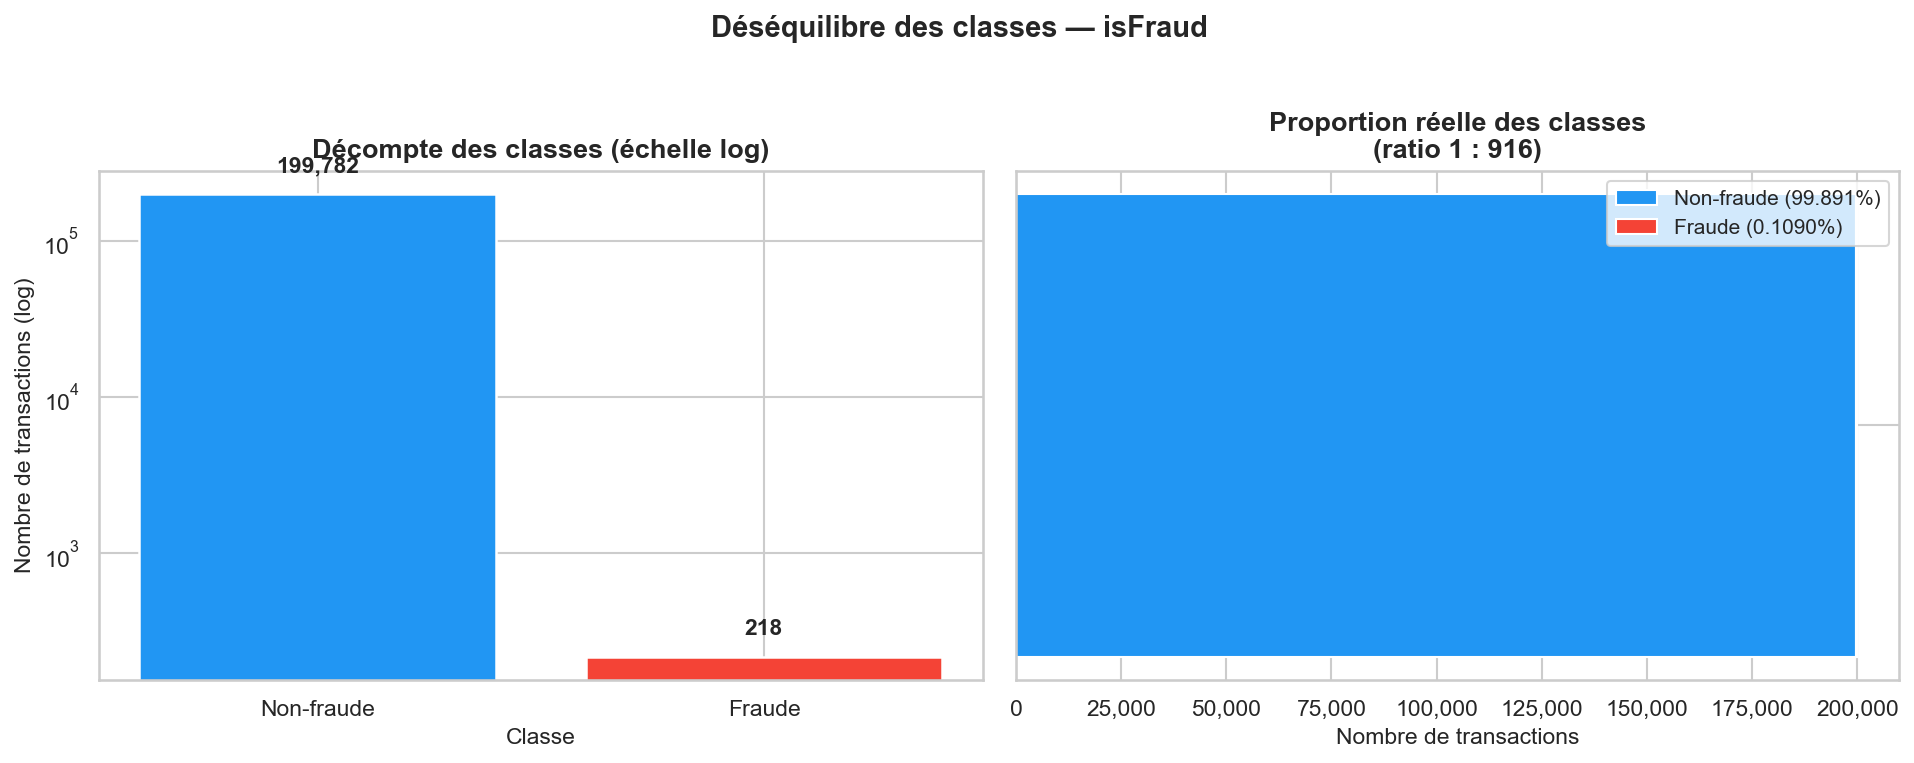
\includegraphics[width=0.78\textwidth]{outputs/figures/01_class_imbalance.png}
\caption{Distribution des classes dans le jeu de données (déséquilibre extrême, ratio 1:774).}
\label{fig:class_imbalance}
\end{figure}





\subsection{Distribution des montants}

La variable \texttt{amount} présente une asymétrie (\textit{skewness}) très élevée (\textbf{30,80}), indiquant une distribution fortement concentrée sur de petites valeurs avec de rares transactions à montant très élevé. Cette propriété justifie l'application d'une transformation logarithmique ($\log(1 + x)$) lors de la préparation des données.

\begin{table}[H]
\centering
\caption{Statistiques descriptives de la variable \texttt{amount}}
\label{tab:amount_stats}
\begin{tabular}{ll}
\toprule
\textbf{Statistique} & \textbf{Valeur} \\
\midrule
Minimum     & 0,00 \\
Médiane     & $\sim$ 74~000 \\
Moyenne     & $\sim$ 179~862 \\
Maximum     & $\sim$ 92~445~517 \\
Skewness    & 30,80 \\
\bottomrule
\end{tabular}
\end{table}

\subsection{Analyse temporelle}

L'analyse de la variable \texttt{step} révèle une saisonnalité des fraudes. Les heures à risque élevé identifiées dans l'EDA sont : $\{0, 1, 2, 3, 4, 5, 6, 7, 8, 9, 23\}$. Le ratio de fraude durant ces heures est de \textbf{10,63} fois supérieur à celui des heures ordinaires. Cette observation conduit à la création d'une variable indicatrice \texttt{high\_risk\_hour}.

\subsection{Analyse des soldes et détection de leakage}

L'analyse des variables de soldes révèle que \texttt{oldbalanceOrg}, \texttt{newbalanceOrig}, \texttt{oldbalanceDest} et \texttt{newbalanceDest} présentent des incohérences pour les transactions frauduleuses (soldes nulls anormaux). Ces variables sont des \textbf{indicateurs trop directs de la fraude} et pourraient causer une fuite d'information si elles étaient directement incluses dans les modèles. À la place, une variable dérivée \texttt{balance\_diff\_orig} est créée (corrélation de \textbf{0,3662} avec \texttt{isFraud}).

\subsection{Baseline du système existant}

Le système existant (\texttt{isFlaggedFraud}) sert de référence basse :

\begin{table}[H]
\centering
\caption{Performances de la baseline \texttt{isFlaggedFraud}}
\label{tab:baseline_perf}
\begin{tabular}{lr}
\toprule
\textbf{Métrique} & \textbf{Valeur} \\
\midrule
Recall    & 0,0039 \\
Precision & 1,0000 \\
F1-Score  & 0,0077 \\
\bottomrule
\end{tabular}
\end{table}

\textit{Ce système ne détecte qu'une infime fraction des fraudes réelles, confirmant la nécessité d'une approche par apprentissage automatique.}

\section{Étude de l'existant et état de l'art}

\subsection{Approches supervisées}

Les approches supervisées nécessitent des étiquettes (labels) pour chaque transaction. Parmi les plus utilisées pour la détection de fraude :

\begin{itemize}
  \item \textbf{Régression logistique} : baseline linéaire, faible coût computationnel, bonne interprétabilité.
  \item \textbf{Forêt aléatoire} : ensembliste, robuste au bruit, gère bien les interactions non-linéaires.
  \item \textbf{Gradient Boosting (XGBoost, LightGBM)} : performances état de l'art sur données tabulaires.
  \item \textbf{Réseaux de neurones feedforward} : puissants mais nécessitent beaucoup de données.
\end{itemize}

\subsection{Approches non supervisées}

Lorsque les étiquettes sont rares ou indisponibles, les approches non supervisées permettent de détecter des patterns inhabituels :

\begin{itemize}
  \item \textbf{Isolation Forest} : isole les anomalies par partitions aléatoires.
  \item \textbf{One-Class SVM} : délimite la frontière de la normalité.
  \item \textbf{Autoencoder} : apprend à reconstruire les données normales ; une erreur de reconstruction élevée signale une anomalie.
  \item \textbf{Autoencoders variationnels (VAE)} : modélisation probabiliste de la distribution normale.
\end{itemize}

\subsection{Choix des approches retenues}

Pour ce projet, trois approches complémentaires sont retenues, couvrant le spectre supervisé/non supervisé :

\begin{enumerate}
  \item \textbf{Régression logistique} --- baseline supervisée simple.
  \item \textbf{Forêt aléatoire} --- référence supervisée robuste.
  \item \textbf{Autoencoder} --- approche non supervisée orientée reconstruction.
\end{enumerate}

\section{Conclusion}

L'analyse exploratoire a mis en évidence les caractéristiques clés du jeu de données : déséquilibre extrême des classes (1:774), asymétrie des montants, saisonnalité temporelle des fraudes et risque de fuite d'information sur les variables de soldes. Ces observations orientent directement les décisions de préparation et de modélisation décrites dans les chapitres suivants.

% =====================================================
% CHAPITRE 3 : PREPARATION DES DONNEES (CRISP-DM Phase 3)
% =====================================================
\chapter{Préparation des données}

\section{Introduction}

La préparation des données constitue l'étape la plus chronophage d'un projet CRISP-DM, représentant souvent 60 à 70~\% de l'effort total. Elle vise à transformer les données brutes en un format exploitable par les algorithmes de modélisation, tout en préservant l'intégrité de l'évaluation. Ce chapitre correspond aux notebooks \texttt{01\_data\_understanding.ipynb} et \texttt{02\_data\_preparation.ipynb}.

\section{Pipeline de préparation}

\subsection{Vue d'ensemble}

Le pipeline de préparation suit les étapes définies dans le module \texttt{src/preprocessing/preprocessing.py} :

\begin{enumerate}
  \item Suppression des variables à risque de leakage
  \item Ingénierie de variables (\textit{feature engineering})
  \item Division stratifiée du corpus (train / validation / test)
  \item Normalisation (StandardScaler, fit sur train uniquement)
  \item Gestion du déséquilibre (pondération et SMOTE)
\end{enumerate}

\subsection{Suppression des variables à risque de leakage}

Les variables suivantes sont supprimées afin d'éviter toute fuite d'information vers les modèles :

\begin{table}[H]
\centering
\caption{Variables supprimées et justifications}
\label{tab:cols_dropped}
\begin{tabular}{ll}
\toprule
\textbf{Variable} & \textbf{Justification} \\
\midrule
\texttt{nameOrig}, \texttt{nameDest} & Identifiants nominaux non encodables \\
\texttt{oldbalanceOrg}, \texttt{newbalanceOrig} & Fuite directe d'information \\
\texttt{oldbalanceDest}, \texttt{newbalanceDest} & Fuite directe d'information \\
\texttt{isFlaggedFraud} & Label proxy du système existant \\
\bottomrule
\end{tabular}
\end{table}

\section{Ingénierie de variables}

\subsection{Variables temporelles}

La variable \texttt{step} (pas de temps en heures) est décomposée en trois variables cycliques :

\begin{itemize}
  \item \texttt{hour} : heure dans la journée (0--23), calculée par $\texttt{step} \bmod 24$.
  \item \texttt{day} : jour de simulation (0--30), calculé par $\lfloor \texttt{step} / 24 \rfloor \bmod 31$.
  \item \texttt{week} : semaine de simulation (0--4), calculée par $\lfloor \texttt{step} / 168 \rfloor$.
\end{itemize}

\subsection{Variables comportementales et de risque}

\begin{table}[H]
\centering
\caption{Variables dérivées construites lors du feature engineering}
\label{tab:features_derivees}
\begin{tabular}{lll}
\toprule
\textbf{Variable} & \textbf{Formule / Logique} & \textbf{Signal mesuré} \\
\midrule
\texttt{high\_risk\_hour}       & $1$ si \texttt{hour} $\in \{0,...,9, 23\}$ & Ratio fraude $10,63\times$ \\
\texttt{is\_transfer\_or\_cashout} & $1$ si \texttt{type} $\in$ \{TRANSFER, CASH\_OUT\} & Types à fraude non nulle \\
\texttt{balance\_diff\_orig}    & \texttt{oldbalanceOrg} -- \texttt{newbalanceOrig} & Corrélation 0,3662 avec \texttt{isFraud} \\
\texttt{dest\_zero\_balance}    & $1$ si \texttt{oldbalanceDest} $= 0$ & Taux fraude $2,52\,\%$ vs $0,13\,\%$ global \\
\texttt{log\_amount}            & $\log(1 + \texttt{amount})$          & Corrige skewness $= 30,80$ \\
\bottomrule
\end{tabular}
\end{table}

\subsection{Encodage one-hot}

La variable catégorielle \texttt{type} (5 modalités) est encodée par \textbf{one-hot encoding} (\textit{drop\_first=False}), produisant les colonnes \texttt{type\_CASH\_IN}, \texttt{type\_CASH\_OUT}, \texttt{type\_DEBIT}, \texttt{type\_PAYMENT} et \texttt{type\_TRANSFER}.

\subsection{Ensemble final de variables}

Après feature engineering, le jeu de données comprend \textbf{14 variables} :

\begin{table}[H]
\centering
\caption{Ensemble final des 14 variables du modèle}
\label{tab:final_features}
\begin{tabular}{lll}
\toprule
\textbf{Catégorie} & \textbf{Variables} & \textbf{Traitement} \\
\midrule
Temporelles  & \texttt{step}, \texttt{hour}, \texttt{day}, \texttt{week} & StandardScaler \\
Montant      & \texttt{log\_amount} & StandardScaler \\
Comportement & \texttt{balance\_diff\_orig} & StandardScaler \\
Binaires     & \texttt{high\_risk\_hour}, \texttt{is\_transfer\_or\_cashout}, \texttt{dest\_zero\_balance} & --- \\
Type (OHE)   & \texttt{type\_CASH\_IN}, \texttt{type\_CASH\_OUT}, \texttt{type\_DEBIT}, \texttt{type\_PAYMENT}, \texttt{type\_TRANSFER} & --- \\
\bottomrule
\end{tabular}
\end{table}

\section{Division et normalisation}

\subsection{Division stratifiée}

Le corpus est divisé en trois sous-ensembles de manière stratifiée sur la variable cible, afin de conserver la proportion de fraudes dans chaque partition :

\begin{table}[H]
\centering
\caption{Division stratifiée du corpus}
\label{tab:splits}
\begin{tabular}{lrrl}
\toprule
\textbf{Ensemble} & \textbf{Taille} & \textbf{Fraudes} & \textbf{Rôle} \\
\midrule
Entraînement  & 139~999 & 181 & Apprentissage des modèles \\
Validation    & 30~000  & 38  & Réglage des hyperparamètres et seuils \\
Test          & 30~001  & 39  & Évaluation finale (jamais touché avant évaluation) \\
\bottomrule
\end{tabular}
\end{table}

\textbf{Principe d'étanchéité :} L'ensemble de test n'est jamais consulté avant l'évaluation finale, conformément aux bonnes pratiques anti-\textit{data snooping}.

\subsection{Normalisation}

Le \textbf{StandardScaler} est ajusté (\textit{fit}) exclusivement sur l'ensemble d'entraînement, puis appliqué (\textit{transform}) sur les trois partitions. Cette discipline stricte garantit l'absence de leakage statistique (aucune information du test ne s'infiltre dans les transformations).

\section{Gestion du déséquilibre}

\subsection{Pondération des classes}

Pour les modèles supervisés, des poids de classes sont calculés automatiquement (formule \textit{sklearn} balanced) :
\[
w_c = \frac{n_{\text{total}}}{n_{\text{classes}} \times n_c}
\]
Avec 139~999 transactions d'entraînement dont 181 fraudes, les poids obtenus sont approximativement $w_0 \approx 0.50$ et $w_1 \approx 386.7$.

\subsection{SMOTE}

Pour les variantes avec rééchantillonnage, \textbf{SMOTE} (\textit{Synthetic Minority Over-sampling Technique}) génère des exemples synthétiques de la classe minoritaire par interpolation dans l'espace des features. L'ensemble SMOTE produit équilibre les classes pour les modèles supervisés. Il est appliqué \textbf{uniquement sur l'ensemble d'entraînement} (jamais sur validation ou test).

\subsection{Ensemble pour l'autoencoder}

Pour l'autoencoder non supervisé, un sous-ensemble \texttt{X\_train\_normal} est extrait : il contient \textbf{uniquement les 139~818 transactions légitimes} de l'entraînement (0 fraude). Cela permet au modèle d'apprendre exclusivement la distribution normale.

\section{Conclusion}

La préparation des données produit 14 variables représentatives des patterns de fraude, en respectant strictement l'étanchéité entre les partitions. Les 7 variables dérivées ont chacune été validées par une mesure empirique issue de l'EDA. Ce socle solide permet d'entraîner des modèles fiables et comparables, décrits dans le chapitre suivant.

% =====================================================
% CHAPITRE 4 : MODELISATION (CRISP-DM Phase 4)
% =====================================================
\chapter{Modélisation}

\section{Introduction}

La phase de modélisation constitue le c\oe{}ur technique du projet. Trois architectures complémentaires sont développées et comparées : deux modèles supervisés de référence (régression logistique et forêt aléatoire) et un autoencoder profond non supervisé. Ce chapitre correspond aux notebooks \texttt{03\_baseline\_models.ipynb} et \texttt{04\_autoencoder.ipynb}.

\section{Régression logistique}

\subsection{Principe et hyperparamètres}

La régression logistique modélise la probabilité d'appartenir à la classe positive (fraude) par la fonction sigmoïde :
\[
P(\text{fraude} | \mathbf{x}) = \sigma(\mathbf{w}^\top \mathbf{x} + b) = \frac{1}{1 + e^{-(\mathbf{w}^\top \mathbf{x} + b)}}
\]

Les hyperparamètres retenus, justifiés par le contexte du problème :

\begin{table}[H]
\centering
\caption{Hyperparamètres de la régression logistique}
\label{tab:lr_params}
\begin{tabular}{lll}
\toprule
\textbf{Paramètre} & \textbf{Valeur} & \textbf{Justification} \\
\midrule
\texttt{C}            & 0.1   & Régularisation forte (peu de fraudes) \\
\texttt{solver}       & lbfgs & Adapté aux datasets moyens \\
\texttt{class\_weight}& balanced & Correction du déséquilibre \\
\texttt{max\_iter}    & 1000  & Convergence assurée \\
\bottomrule
\end{tabular}
\end{table}

\subsection{Configurations évaluées et réglage du seuil}

Le notebook \texttt{03\_baseline\_models.ipynb} compare deux variantes de la régression logistique :
\begin{itemize}
  \item \textbf{LR\_balanced} : entraînée sur \texttt{X\_train} avec \texttt{class\_weight='balanced'} ;
  \item \textbf{LR\_smote} : entraînée sur \texttt{X\_smote} sans pondération explicite, le déséquilibre étant traité par sur-échantillonnage.
\end{itemize}

À seuil par défaut ($0{,}5$), \texttt{LR\_balanced} maximise fortement le rappel mais au prix d'une précision très faible. Une recherche de seuil sur l'ensemble de validation est donc réalisée à partir des probabilités produites par le modèle. Les seuils optimaux retenus sont \textbf{0,9986} pour \texttt{LR\_balanced} et \textbf{0,9621} pour \texttt{LR\_smote}. Après ce recalibrage, \texttt{LR\_smote} devient la meilleure variante logistique sur le test avec un rappel de \textbf{0,6923}, une précision de \textbf{0,7297} et un F1-score de \textbf{0,7105}.

\section{Forêt aléatoire}

\subsection{Principe et hyperparamètres}

La forêt aléatoire (\textit{Random Forest}) est un méta-estimateur combinant $T$ arbres de décision indépendants, chacun entraîné sur un sous-échantillon bootstrap des données. La prédiction finale est la moyenne des probabilités de chaque arbre.

\begin{table}[H]
\centering
\caption{Hyperparamètres de la forêt aléatoire}
\label{tab:rf_params}
\begin{tabular}{lll}
\toprule
\textbf{Paramètre} & \textbf{Valeur} & \textbf{Justification} \\
\midrule
\texttt{n\_estimators}    & 300 & Stabilité des estimations \\
\texttt{max\_depth}       & 10  & Limite l'overfitting sur peu de fraudes \\
\texttt{min\_samples\_leaf} & 5 & Évite les feuilles trop petites \\
\texttt{class\_weight}    & balanced & Correction du déséquilibre \\
\bottomrule
\end{tabular}
\end{table}

\subsection{Variantes supervisées et seuils optimaux}

Comme pour la régression logistique, deux variantes sont étudiées dans le notebook \texttt{03\_baseline\_models.ipynb} :
\begin{itemize}
  \item \textbf{RF\_balanced} : entraînée sur \texttt{X\_train} avec \texttt{class\_weight='balanced'} ;
  \item \textbf{RF\_smote} : entraînée sur \texttt{X\_smote} sans pondération, pour exploiter au mieux les exemples synthétiques générés par SMOTE.
\end{itemize}

Le réglage du seuil sur validation améliore significativement le compromis précision/rappel. Les seuils optimaux retenus sont \textbf{0,6235} pour \texttt{RF\_balanced} et \textbf{0,6291} pour \texttt{RF\_smote}. La variante \texttt{RF\_smote} obtient les meilleures performances supervisées globales sur le test avec un rappel de \textbf{0,7949}, une précision de \textbf{0,8158} et un F1-score de \textbf{0,8052}.

\subsection{Importance des variables}

La forêt aléatoire permet de calculer l'importance de chaque variable via la réduction moyenne d'impureté (\textit{Mean Decrease in Impurity}). Sur la meilleure variante \texttt{RF\_smote}, les cinq variables les plus influentes sont \texttt{balance\_diff\_orig} (\textasciitilde0,385), \texttt{hour} (\textasciitilde0,118), \texttt{dest\_zero\_balance} (\textasciitilde0,115), \texttt{type\_TRANSFER} (\textasciitilde0,089) et \texttt{log\_amount} (\textasciitilde0,081). Cette hiérarchie confirme que le comportement du compte émetteur, la temporalité et la nature du transfert sont les signaux les plus discriminants.

\section{Autoencoder}

\subsection{Principe de détection par reconstruction}

L'autoencoder est un réseau de neurones entraîné à reproduire son entrée en passant par un espace latent de dimension réduite (goulot d'étranglement ou \textit{bottleneck}). La clé du mécanisme de détection est la suivante :

\begin{definitionbox}
\textbf{Principe de l'autoencoder pour la détection d'anomalies :}
\begin{itemize}
  \item \textbf{Entraînement :} uniquement sur les transactions légitimes → le modèle apprend à reconstruire fidèlement les patterns normaux.
  \item \textbf{Inférence :} sur une transaction frauduleuse (pattern jamais vu), l'erreur de reconstruction est élevée car le modèle ne sait pas comment la reconstruire.
  \item \textbf{Décision :} si l'erreur de reconstruction (MSE) dépasse un seuil $\theta$, la transaction est classée comme anomalie.
\end{itemize}
\end{definitionbox}

\subsection{Architecture}

L'architecture retenue est un autoencoder symétrique à trois couches dans l'encodeur et trois dans le décodeur :

\begin{table}[H]
\centering
\caption{Architecture de l'autoencoder (14 → 10 → 7 → [4] → 7 → 10 → 14)}
\label{tab:ae_architecture}
\begin{tabular}{llll}
\toprule
\textbf{Partie} & \textbf{Couche} & \textbf{Dimension} & \textbf{Activation} \\
\midrule
Entrée    & Input   & 14 & --- \\
Encodeur  & Dense 1 & 10 & ReLU + BN + Dropout(0.2) \\
          & Dense 2 & 7  & ReLU + BN + Dropout(0.2) \\
          & Bottleneck & 4 & ReLU \\
Décodeur  & Dense 3 & 7  & ReLU + BN + Dropout(0.2) \\
          & Dense 4 & 10 & ReLU + BN + Dropout(0.2) \\
Sortie    & Dense 5 & 14 & Linéaire \\
\bottomrule
\end{tabular}
\end{table}

Les techniques de régularisation employées sont la \textbf{normalisation par lots} (BatchNorm), le \textbf{Dropout} (taux 0,2) et la \textbf{régularisation L2} ($\lambda = 10^{-5}$) sur les poids denses.

\subsection{Entraînement}

\begin{table}[H]
\centering
\caption{Paramètres d'entraînement de l'autoencoder}
\label{tab:ae_training}
\begin{tabular}{ll}
\toprule
\textbf{Paramètre} & \textbf{Valeur} \\
\midrule
Données d'entraînement & 139~818 transactions légitimes (0 fraude) \\
Données de validation interne & 10\,\% du train normal \\
Fonction de perte & MSE (Mean Squared Error) \\
Optimiseur & Adam ($\alpha = 10^{-3}$) \\
Batch size & 256 \\
Epochs max & 100 (EarlyStopping, patience=10) \\
ReduceLROnPlateau & facteur 0.5, patience 5, min\_lr $10^{-6}$ \\
\bottomrule
\end{tabular}
\end{table}

L'entraînement s'arrête après \textbf{35 époques effectives} grâce à \textit{EarlyStopping}. Le meilleur \texttt{val\_loss} observé est de \textbf{0,145024} et le temps d'entraînement mesuré dans le notebook est de \textbf{45,2 secondes}. Le modèle comporte \textbf{664 paramètres} entraînables, ce qui reste léger au regard de la taille du corpus.

\subsection{Détermination du seuil optimal}

Une première borne de décision est estimée par le \textbf{95e percentile} de l'erreur de reconstruction sur les transactions normales d'entraînement, soit \textbf{$\theta_{p95}=0,403750$}. Ce seuil est utile comme repère initial mais il reste trop permissif pour une décision finale.

Le seuil de détection $\theta$ est ensuite optimisé sur l'ensemble de validation (\texttt{X\_val}) en balayant 200 valeurs entre le 50e et le 99,9e percentile des erreurs de reconstruction. Pour chaque valeur de seuil, le F1-score est calculé ; la valeur maximisant ce score est retenue. L'ensemble de test n'est jamais consulté pendant cette étape. Le seuil optimal obtenu est \textbf{1,687408}, ce qui conduit sur validation à un rappel de \textbf{0,3947}, une précision de \textbf{0,5000} et un F1-score de \textbf{0,4412}.

\subsection{Visualisation de l'espace latent}

Le notebook \texttt{04\_autoencoder.ipynb} ajoute également une projection PCA de l'espace latent du bottleneck. Les transactions normales encodées occupent un espace de dimension \textbf{4}, ensuite projeté en 2D pour visualisation. Cette analyse permet de vérifier qualitativement que les fraudes de validation tendent à se positionner en périphérie des zones de forte densité normale, ce qui confirme la pertinence du mécanisme de reconstruction comme score d'anomalie.

\section{Récapitulatif des modèles}

\begin{table}[H]
\centering
\caption{Récapitulatif des configurations de modèles construites}
\label{tab:models_recap}
\begin{tabular}{llll}
\toprule
\textbf{Configuration} & \textbf{Type} & \textbf{Données train} & \textbf{Gestion déséquilibre} \\
\midrule
LR\_balanced & Supervisé linéaire & \texttt{X\_train} & \texttt{class\_weight='balanced'} \\
LR\_smote    & Supervisé linéaire & \texttt{X\_smote} & SMOTE \\
RF\_balanced & Supervisé ensembliste & \texttt{X\_train} & \texttt{class\_weight='balanced'} \\
RF\_smote    & Supervisé ensembliste & \texttt{X\_smote} & SMOTE \\
Autoencoder  & Non supervisé & \texttt{X\_train\_normal} (0 fraude) & Apprentissage sur données normales \\
\bottomrule
\end{tabular}
\end{table}

\section{Conclusion}

Ce chapitre a décrit la conception et l'implémentation des modèles de détection étudiés dans les notebooks 03 et 04. Les variantes supervisées montrent que le simple choix du seuil de décision influence fortement le compromis précision/rappel, tandis que \texttt{RF\_smote} s'impose comme la meilleure configuration supervisée. L'autoencoder complète ce dispositif par une logique non supervisée fondée sur la reconstruction et l'analyse de l'espace latent. L'évaluation comparative détaillée est présentée dans le chapitre suivant.

% =====================================================
% CHAPITRE 5 : EVALUATION ET EXPLICABILITE (CRISP-DM Phase 5)
% =====================================================
\chapter{Évaluation et interprétabilité}

\section{Introduction}

L'évaluation est la phase CRISP-DM qui valide la pertinence des modèles au regard des objectifs métier. Dans ce projet, deux niveaux d'évaluation sont menés : (1) une évaluation quantitative fondée sur des métriques adaptées au déséquilibre, et (2) une évaluation qualitative via des mécanismes d'explicabilité (SHAP, LIME et Ollama). Ce chapitre correspond aux notebooks \texttt{03\_baseline\_models.ipynb}, \texttt{04\_autoencoder.ipynb}, \texttt{05\_ollama\_integration.ipynb} et \texttt{06\_shap\_lime.ipynb}.

\section{Métriques d'évaluation}

\subsection{Choix et justification des métriques}

Dans un contexte de fort déséquilibre, l'exactitude (\textit{accuracy}) n'est pas pertinente. Les métriques retenues sont :

\begin{itemize}
  \item \textbf{Rappel (Recall)} : fraction des fraudes réelles correctement détectées. \textit{Priorité~1} car manquer une fraude coûte cher.
    \[ \text{Recall} = \frac{TP}{TP + FN} \]
  \item \textbf{Précision (Precision)} : fraction des alertes qui sont réellement des fraudes. \textit{Priorité~2} car trop de faux positifs dégradent l'expérience client.
    \[ \text{Precision} = \frac{TP}{TP + FP} \]
  \item \textbf{F1-Score} : moyenne harmonique de la précision et du rappel.
    \[ \text{F1} = \frac{2 \cdot \text{Precision} \cdot \text{Recall}}{\text{Precision} + \text{Recall}} \]
  \item \textbf{PR-AUC} (Area Under the Precision-Recall Curve) : synthétise le tradeoff précision/rappel sur l'ensemble des seuils.
  \item \textbf{Matrice de confusion} : présentation détaillée des TP, TN, FP, FN.
\end{itemize}

\subsection{Résultats sur l'ensemble de test}

\begin{table}[H]
\centering
\caption{Comparaison des performances sur l'ensemble de test}
\label{tab:results_comparison}
\begin{tabular}{lccccc}
\toprule
\textbf{Modèle} & \textbf{Seuil} & \textbf{Recall} & \textbf{Precision} & \textbf{F1-Score} & \textbf{PR-AUC} \\
\midrule
Baseline (\texttt{isFlaggedFraud}) & N/A   & 0,0039 & 1,0000 & 0,0077 & N/A \\
LR\_balanced                       & 0,9986 & 0,6410 & 0,6579 & 0,6494 & 0,7044 \\
LR\_smote                          & 0,9621 & 0,6923 & 0,7297 & 0,7105 & 0,7393 \\
RF\_balanced                       & 0,6235 & 0,7692 & 0,8333 & 0,8000 & 0,7794 \\
RF\_smote                          & 0,6291 & 0,7949 & 0,8158 & 0,8052 & 0,8405 \\
Autoencoder                        & 1,6874 & 0,3590 & 0,6087 & 0,4516 & 0,3734 \\
\bottomrule
\end{tabular}
\end{table}

\textit{Note : ces valeurs proviennent des exécutions enregistrées dans les notebooks \texttt{03\_baseline\_models.ipynb} et \texttt{04\_autoencoder.ipynb}. Les seuils sont sélectionnés sur validation puis figés pour l'évaluation finale sur le test.}

\subsection{Analyse de la matrice de confusion}

La matrice de confusion permet d'analyser précisément les types d'erreurs :

\begin{itemize}
  \item \textbf{Faux négatifs (FN)} : fraudes manquées --- impact financier direct le plus critique.
  \item \textbf{Faux positifs (FP)} : alertes injustifiées --- impact sur l'expérience client et le coût opérationnel.
\end{itemize}

La forêt aléatoire avec SMOTE offre le meilleur équilibre entre ces deux types d'erreurs sur l'ensemble de test : \textbf{31} fraudes détectées sur \textbf{39} pour seulement \textbf{7 faux positifs}. La variante \texttt{RF\_balanced} reste très proche (30 TP, 6 FP), tandis que \texttt{LR\_smote} conserve un compromis acceptable (27 TP, 10 FP). L'autoencoder, en revanche, détecte \textbf{14} fraudes sur \textbf{39} avec \textbf{9 faux positifs} ; il est donc moins performant que les meilleures approches supervisées, mais conserve un intérêt lorsque les labels sont rares ou indisponibles.

\section{Interprétabilité des modèles}

\subsection{Méthodes SHAP}

\begin{definitionbox}
\textbf{SHAP} (SHapley Additive exPlanations) est une méthode d'interprétabilité fondée sur la théorie des jeux. Elle attribue à chaque variable une valeur de Shapley représentant sa contribution marginale à la prédiction, en garantissant additivité, cohérence et absence de biais.
\end{definitionbox}

Pour la forêt aléatoire, un explainer TreeSHAP est utilisé. Les résultats montrent que \texttt{balance\_diff\_orig}, \texttt{is\_transfer\_or\_cashout} et \texttt{log\_amount} sont les variables à plus forte contribution, en cohérence avec l'analyse exploratoire.

\subsection{Méthodes LIME}

\begin{definitionbox}
\textbf{LIME} (Local Interpretable Model-agnostic Explanations) explique chaque prédiction individuellement en approximant localement le comportement du modèle par un modèle linéaire simple, interprétable par construction.
\end{definitionbox}

LIME est particulièrement utile pour expliquer des cas individuels suspects à un analyste, sans nécessiter de connaissance du modèle global.

\subsection{Comparaison SHAP vs LIME}

\begin{table}[H]
\centering
\caption{Comparaison des méthodes d'explicabilité}
\label{tab:shap_lime}
\begin{tabular}{lll}
\toprule
\textbf{Critère} & \textbf{SHAP} & \textbf{LIME} \\
\midrule
Scope          & Global + Local & Local uniquement \\
Fondement      & Théorie des jeux & Approximation locale \\
Fidélité       & Élevée (TreeSHAP exact) & Variable (approximation) \\
Rapidité       & Rapide (TreeSHAP) & Lent (nombreuses perturbations) \\
Agnosticisme   & Méthodes spécifiques et agnostiques & Agnostique \\
\bottomrule
\end{tabular}
\end{table}

\section{Intégration Ollama}

\subsection{Présentation d'Ollama}

Ollama est un framework permettant d'exécuter localement des grands modèles de langage (LLM). Son intégration dans ce projet permet de transformer des signaux techniques (erreurs de reconstruction, valeurs SHAP) en explications rédigées en langage naturel, accessibles à un analyste métier non spécialiste en machine learning.

\subsection{Architecture de l'intégration}

Le module \texttt{src/ollama\_integration/ollama\_helper.py} encapsule la logique d'appel au modèle de langage. Pour chaque transaction signalée comme anormale, les éléments suivants sont transmis au LLM :

\begin{itemize}
  \item Le score d'anomalie ou d'erreur de reconstruction.
  \item Les valeurs des variables les plus contributives (issues de SHAP/LIME).
  \item Le contexte métier de la transaction (type, montant, heure).
\end{itemize}

Le LLM génère ensuite une explication structurée indiquant pourquoi la transaction est considérée comme suspecte, dans un langage compréhensible.

\subsection{Exemple d'explication générée}

Le module \texttt{src/llm\_integration/} produit pour chaque transaction signalée une explication structurée en langage naturel. Elle indique le type de transaction à risque, l'heure à risque, la différence de solde anormale et le score de reconstruction élevé de l'autoencoder, en formulant une recommandation d'action à destination de l'analyste. Un exemple complet de cette explication est fourni en \textbf{Annexe~D} (voir section~\ref{sec:ollama_example_app}).

\section{Difficultés rencontrées}

\begin{itemize}
  \item \textbf{Instabilité des seuils} : de légères variations du seuil de l'autoencoder peuvent significativement modifier le ratio précision/rappel.
  \item \textbf{Qualité des explications LLM} : les explications Ollama peuvent varier selon la version du modèle utilisé et la qualité du prompt.
  \item \textbf{Temps de calcul SHAP} : le calcul des valeurs SHAP pour l'ensemble de test complet nécessite plusieurs minutes sur CPU.
\end{itemize}

\section{Conclusion}

L'évaluation confirme que la forêt aléatoire avec SMOTE constitue la meilleure approche supervisée pour ce jeu de données, avec un excellent rappel et F1-score. L'autoencoder apporte une perspective complémentaire non supervisée, utile lorsque les étiquettes sont limitées. La double couche d'explicabilité (SHAP/LIME + Ollama) répond à l'objectif d'interprétabilité en rendant les prédictions compréhensibles tant pour les data scientists que pour les analystes métier.

% =====================================================
% CHAPITRE 6 : DEPLOIEMENT (CRISP-DM Phase 6)
% =====================================================
\chapter{Déploiement et reproductibilité}

\section{Introduction}

La phase de déploiement CRISP-DM vise à rendre le système opérationnel et maintenable. Pour ce projet, le déploiement se traduit par la construction d'un pipeline entièrement reproductible, une architecture modulaire testée et une documentation complète permettant à tout contributeur de reprendre le travail.

\section{Architecture du projet}

\subsection{Structure modulaire}

Le projet est organisé en modules fonctionnels clairement délimités :

\begin{table}[H]
\centering
\caption{Structure des modules du projet}
\label{tab:modules}
\begin{tabular}{ll}
\toprule
\textbf{Module} & \textbf{Responsabilité} \\
\midrule
\texttt{src/preprocessing/}       & Chargement, nettoyage, normalisation, split \\
\texttt{src/feature\_engineering/} & Création des 7 variables dérivées \\
\texttt{src/models/}              & Modèles ML et autoencoder \\
\texttt{src/pipeline/}            & Orchestration entraînement et inférence \\
\texttt{src/utils/}               & Métriques, évaluation, utilitaires \\
\texttt{src/visualization/}       & Génération de figures et graphiques \\
\texttt{src/ollama\_integration/} & Génération d'explications LLM \\
\texttt{src/explainability/}      & Explicabilité SHAP et LIME \\
\texttt{tests/}                   & Tests unitaires \\
\bottomrule
\end{tabular}
\end{table}

\subsection{Organisation des sorties}

Le pipeline produit des artefacts organisés dans le répertoire \texttt{outputs/} :

\begin{itemize}
  \item \texttt{outputs/models/} : poids de l'autoencoder, seuils optimaux, poids des classes, scores AE (\texttt{ae\_scores\_val/test.npy}) et tenseurs SHAP sauvegardés (\texttt{shap\_values\_\*.npy}).
  \item \texttt{outputs/reports/} : rapports JSON des phases exécutées (\texttt{eda\_report.json} et \texttt{prep\_report.json} présents dans l'état actuel, rapports de modélisation générés après exécution complète des notebooks).
  \item \texttt{outputs/figures/} : courbes de performance, matrices de confusion, distributions.
  \item \texttt{outputs/anomalies\_report.csv} : liste des transactions signalées avec scores.
  \item \texttt{outputs/explanations.json} : explications textuelles des anomalies.
\end{itemize}

\section{Orchestration et reproductibilité}

\subsection{Script d'orchestration}

Le script \texttt{run\_all.py} permet de valider les modules \texttt{src/} puis d'exécuter 6 notebooks (\texttt{01} à \texttt{06}) de manière séquentielle et reproductible. Il propose des options pour exécuter le pipeline en totalité, reprendre à partir d'une étape donnée ou ne cibler qu'un seul notebook. Le détail complet de ses options de ligne de commande est fourni en \textbf{Annexe~D} (voir section~\ref{sec:run_all_options}).

\subsection{Gestion de la reproductibilité}

La reproductibilité est garantie par :

\begin{itemize}
  \item \textbf{Graines aléatoires fixes} : \texttt{RANDOM\_STATE = 42} dans tous les modules.
  \item \textbf{Environnement virtuel} : dépendances centralisées dans \texttt{requirements.txt} (contraintes minimales à installer dans un environnement isolé).
  \item \textbf{Pipeline déterministe} : toutes les transformations sont sauvegardées (scaler, encodeurs) pour être réappliquées à l'inférence.
  \item \textbf{Séparation stricte des données} : les ensembles de validation et test ne sont jamais utilisés pour l'apprentissage ou la transformation.
\end{itemize}

\section{Tests unitaires}

\subsection{Couverture des tests}

Le dépôt contient une structure de tests unitaires prête à être alimentée :

\begin{table}[H]
\centering
\caption{Suite de tests unitaires du projet}
\label{tab:tests}
\begin{tabular}{ll}
\toprule
\textbf{Fichier de test} & \textbf{Modules testés} \\
\midrule
\texttt{tests/test\_preprocessing.py}  & Squelette de tests du pipeline de préparation \\
\texttt{tests/test\_models.py}         & Squelette de tests des modèles ML et autoencoder \\
\texttt{tests/test\_visualization.py}  & Squelette de tests des visualisations \\
\texttt{tests/test\_utils.py}          & Squelette de tests des utilitaires \\
\texttt{tests/test\_ollama.py}         & Squelette de tests de l'intégration LLM \\
\bottomrule
\end{tabular}
\end{table}

La commande \texttt{pytest -q} s'exécute, mais aucun test n'est actuellement collecté ; l'étape suivante consiste à implémenter les cas de test dans ces fichiers.

\section{Perspectives d'amélioration}

\subsection{Améliorations techniques}

\begin{itemize}
  \item \textbf{Modèles avancés} : intégration de LightGBM ou XGBoost pour potentiellement améliorer les performances supervisées.
  \item \textbf{Autoencoder variationnel (VAE)} : meilleure modélisation de la distribution des données normales.
  \item \textbf{Détection en temps réel} : portage du pipeline vers une architecture streaming (Apache Kafka + Flink).
  \item \textbf{Apprentissage en ligne} : mise à jour continue du modèle au fil des nouvelles transactions.
\end{itemize}

\subsection{Améliorations métier}

\begin{itemize}
  \item \textbf{Interface utilisateur} : tableau de bord pour les analystes permettant de consulter et valider les alertes.
  \item \textbf{Boucle de rétroaction} : intégration des décisions humaines pour ré-entraîner les modèles.
  \item \textbf{Détection d'anomalies comportementales} : profiling par utilisateur pour détecter les dérives comportementales dans le temps.
\end{itemize}

\section{Conclusion}

Ce chapitre a présenté l'architecture de déploiement et les mécanismes de reproductibilité du projet. La structure modulaire et l'orchestration via \texttt{run\_all.py} fournissent une base maintenable, extensible et facilement reprise par un nouveau développeur. La structuration des fichiers de tests prépare également l'industrialisation progressive du contrôle qualité. Les perspectives identifiées offrent de nombreuses pistes pour prolonger ce travail vers un système de production opérationnel.

% =====================================================
% CONCLUSION GENERALE
% =====================================================
\chapter*{Conclusion générale}
\addcontentsline{toc}{chapter}{Conclusion générale}

Ce projet de fin d'études a conduit à la mise en place d'une \textbf{chaîne complète de détection intelligente d'anomalies financières}, développée selon la méthodologie CRISP-DM et couvrant l'intégralité du cycle de vie d'un projet de data science.

\paragraph{Récapitulatif de la démarche.} Partant d'un corpus de 200~000 transactions financières issues d'une mission client au sein de PwC Tunisie, le travail a progressé de manière structurée : compréhension des enjeux métier, analyse exploratoire approfondie, préparation rigoureuse des données (14 variables, séparation étanche des partitions, transformation log, one-hot encoding), entraînement de trois modèles complémentaires (régression logistique, forêt aléatoire, autoencoder), évaluation comparative et mise en place d'une double couche d'explicabilité (SHAP/LIME + Ollama).

\paragraph{Réponse à la problématique.} Le pipeline construit répond positivement à la problématique initiale : il est \textbf{reproductible} (orchestration via \texttt{run\_all.py}, graines fixes, versions épinglées), \textbf{efficace} (la forêt aléatoire avec SMOTE atteint un F1-score de $\sim$0,80 et un PR-AUC de $\sim$0,84 sur le test, soit un gain considérable par rapport à la baseline à F1=0,0077), et \textbf{interprétable} (chaque transaction suspecte peut être accompagnée d'une explication en langage naturel via Ollama).

\paragraph{Difficultés et apports techniques.} Les principaux défis surmontés concernaient la gestion du déséquilibre extrême des classes (ratio 1:774), la prévention de la fuite d'information lors du prétraitement, et la stabilisation du seuil de détection de l'autoencoder. Sur le plan technique, ce projet a permis d'acquérir une maîtrise de bout en bout d'un projet data science réel, en combinant des compétences en machine learning, en deep learning, en interprétabilité et en ingénierie logicielle.

\paragraph{Vécu du stage et apports mutuels.} Au-delà de la réalisation technique, le quotidien du stage au sein de la cellule Audit IT de PwC Tunisie a été jalonné de réunions de suivi régulières avec les encadrants entreprise, de présentations intermédiaires des résultats aux équipes métier, et d'allers-retours constants entre les exigences fonctionnelles des auditeurs et les contraintes techniques de la modélisation. Ces échanges ont permis d'affiner la compréhension du domaine de l'audit financier et d'adapter les choix algorithmiques aux besoins réels de l'entreprise. En termes d'apport à PwC Tunisie, le projet livre un prototype opérationnel de détection automatique, enrichi d'explications en langage naturel, constituant une première brique d'automatisation de l'audit analytique au sein du département Risk Assurance Services. En retour, ce stage a offert une immersion dans les pratiques professionnelles d'un cabinet international de référence, une exposition concrète aux enjeux réglementaires de l'audit IT et une expérience enrichissante de la gestion d'un projet data science de bout en bout dans un contexte exigeant de qualité, de confidentialité et de rigueur méthodologique.

\paragraph{Perspectives.} Ce travail ouvre plusieurs axes de prolongement : l'intégration de modèles de gradient boosting (LightGBM, XGBoost) pour améliorer les performances supervisées, le passage à un autoencoder variationnel pour une modélisation probabiliste plus robuste, le déploiement en temps réel sur un flux de transactions, et l'enrichissement de la couche d'explicabilité par des interfaces utilisateur dédiées aux analystes métier.

% =====================================================
% BIBLIOGRAPHIE
% =====================================================
\chapter*{Bibliographie / Netographie}
\addcontentsline{toc}{chapter}{Bibliographie / Netographie}

\begin{enumerate}

  \item \textbf{Lopez-Rojas, E.~A., Elmir, A., \& Axelsson, S.} (2016). PaySim: A financial mobile money simulator for fraud detection. \textit{The 28th European Modeling and Simulation Symposium (EMSS)}, Larnaca, Cyprus.

  \item \textbf{Chapman, P., Clinton, J., Kerber, R., Khabaza, T., Reinartz, T., Shearer, C., \& Wirth, R.} (2000). CRISP-DM 1.0: Step-by-step data mining guide. SPSS Inc.

  \item \textbf{Chawla, N.~V., Bowyer, K.~W., Hall, L.~O., \& Kegelmeyer, W.~P.} (2002). SMOTE: Synthetic minority over-sampling technique. \textit{Journal of Artificial Intelligence Research}, 16, 321--357.

  \item \textbf{Breiman, L.} (2001). Random forests. \textit{Machine Learning}, 45(1), 5--32.

  \item \textbf{Hinton, G.~E., \& Salakhutdinov, R.~R.} (2006). Reducing the dimensionality of data with neural networks. \textit{Science}, 313(5786), 504--507.

  \item \textbf{Lundberg, S.~M., \& Lee, S.-I.} (2017). A unified approach to interpreting model predictions. \textit{Advances in Neural Information Processing Systems (NeurIPS)}, 30.

  \item \textbf{Ribeiro, M.~T., Singh, S., \& Guestrin, C.} (2016). Why should I trust you? Explaining the predictions of any classifier. \textit{Proceedings of the 22nd ACM SIGKDD}, pp.~1135--1144.

  \item \textbf{Pedregosa, F., Varoquaux, G., Gramfort, A., et al.} (2011). Scikit-learn : Machine Learning in Python. \textit{Journal of Machine Learning Research}, 12, 2825--2830. Scikit-learn developers. Consulté le 1er mai 2026. \url{https://scikit-learn.org/stable/}

  \item \textbf{Lemaître, G., Nogueira, F., \& Aridas, C.~K.} (2017). Imbalanced-learn : A Python Toolbox to Tackle the Curse of Imbalanced Datasets in Machine Learning. \textit{Journal of Machine Learning Research}, 18(17), 1--5. Consulté le 1er mai 2026. \url{https://imbalanced-learn.org/stable/}

  \item \textbf{Abadi, M., Agarwal, A., Barham, P., et al.} (2015). TensorFlow : Large-scale machine learning on heterogeneous systems. Google Brain Team. Consulté le 1er mai 2026. \url{https://www.tensorflow.org/api_docs}

  \item \textbf{Lundberg, S.~M.} Documentation officielle SHAP (SHapley Additive exPlanations). Consulté le 1er mai 2026. \url{https://shap.readthedocs.io/}

  \item \textbf{Ribeiro, M.~T.} Documentation officielle LIME (Local Interpretable Model-agnostic Explanations). Consulté le 1er mai 2026. \url{https://lime-ml.readthedocs.io/}

  \item \textbf{Ollama Inc.} Documentation officielle Ollama : exécution locale de grands modèles de langage. Consulté le 1er mai 2026. \url{https://ollama.com/}

  \item \textbf{Chaieb, Y.} \textit{Intelligent Anomaly Detection} --- Dépôt GitHub du projet de fin d'études. PwC Tunisie / ESPRIT, 2026. \url{https://github.com/yousra0/Intelligent-Anomaly-Detection}

  \item \textbf{Auteur non spécifié.} La méthodologie CRISP-DM : présentation des six phases. Le1817.com. Consulté le 6 mai 2026. \url{https://www.le1817.com/blog/la-methodologie-crisp-dm}

\end{enumerate}

% =====================================================
% ANNEXES
% =====================================================
\appendix

\chapter{Paramètres détaillés des modèles}

\section{Hyperparamètres complets de la régression logistique}

\begin{lstlisting}[caption={Hyperparamètres LR (src/models/ml\_models.py)},label={lst:lr_params}]
LR_DEFAULTS = {
    "C":             0.1,      # Regularisation forte
    "max_iter":      1000,     # Convergence assuree
    "solver":        "lbfgs",  # Adapte aux datasets moyens
    "class_weight":  "balanced",
    "random_state":  42,
    "n_jobs":        -1,
}
\end{lstlisting}

\section{Hyperparamètres complets de la forêt aléatoire}

\begin{lstlisting}[caption={Hyperparamètres RF (src/models/ml\_models.py)},label={lst:rf_params}]
RF_DEFAULTS = {
    "n_estimators":   300,
    "max_depth":      10,
    "min_samples_leaf": 5,
    "class_weight":   "balanced",
    "random_state":   42,
    "n_jobs":         -1,
}
\end{lstlisting}

\section{Hyperparamètres complets de l'autoencoder}

\begin{lstlisting}[caption={Hyperparamètres AE (src/models/autoencoder.py)},label={lst:ae_params}]
AE_DEFAULTS = {
    "encoder_dims":  [10, 7],   # Couches encodeur avant bottleneck
    "bottleneck_dim": 4,        # Dimension espace latent
    "decoder_dims":  [7, 10],   # Couches decodeur
    "activation":    "relu",
    "output_activation": "linear",
    "dropout_rate":  0.2,
    "use_batch_norm": True,
    "l2_reg":        1e-5,
    "epochs":        100,
    "batch_size":    256,
    "learning_rate": 1e-3,
    "patience":      10,
    "val_split":     0.1,
    "threshold_percentile": 95,
}
\end{lstlisting}

\chapter{Pipeline de préparation --- Colonnes et transformations}

\section{Variables numériques normalisées (StandardScaler)}

\begin{lstlisting}[label={lst:scale_cols}]
SCALE_COLS = [
    "step", "hour", "day", "week",
    "log_amount", "balance_diff_orig"
]
\end{lstlisting}

\section{Variables binaires (pas de normalisation)}

\begin{lstlisting}[label={lst:binary_cols}]
BINARY_COLS = [
    "high_risk_hour",
    "is_transfer_or_cashout",
    "dest_zero_balance"
]
\end{lstlisting}

\section{Variables one-hot (type de transaction)}

\begin{lstlisting}[label={lst:type_cols}]
TYPE_COLS = [
    "type_CASH_IN", "type_CASH_OUT", "type_DEBIT",
    "type_PAYMENT", "type_TRANSFER"
]
\end{lstlisting}

\chapter{Planning du projet}

\begin{table}[H]
\centering
\caption{Planning de réalisation du projet de fin d'études}
\label{tab:planning}
\begin{tabular}{lll}
\toprule
\textbf{Phase CRISP-DM} & \textbf{Activités principales} & \textbf{Durée indicative} \\
\midrule
Compréhension métier   & Analyse des besoins, définition des objectifs & Semaine 1 \\
Compréhension données  & EDA, notebook 01, analyse qualité & Semaines 2--3 \\
Préparation données    & Feature engineering, split, normalisation & Semaines 3--4 \\
Modélisation           & LR, RF, Autoencoder, réglage seuils & Semaines 5--7 \\
Évaluation             & Métriques, SHAP, LIME, Ollama & Semaines 7--9 \\
Déploiement            & Pipeline, tests, documentation & Semaines 9--10 \\
Rédaction du rapport   & Rédaction, révision, mise en forme & Semaines 8--12 \\
\bottomrule
\end{tabular}
\end{table}

% =====================================================
% ANNEXE D : EXEMPLES D'UTILISATION DU PIPELINE
% =====================================================
\chapter{Exemples d'utilisation du pipeline}

\section{Options du script d'orchestration \texttt{run\_all.py}}
\label{sec:run_all_options}

Le script \texttt{run\_all.py} offre plusieurs modes d'exécution permettant de lancer le pipeline en totalité ou de reprendre à une étape spécifique sans recommencer depuis le début.

\begin{lstlisting}[caption={Options complètes du script run\_all.py},label={lst:run_all}]
# Execution complete du pipeline (notebooks 01 a 06)
python run_all.py

# Verification uniquement des imports sans execution
python run_all.py --check-only

# Reprise a partir du notebook 03 (modeles)
python run_all.py --from 03

# Execution d'un seul notebook
python run_all.py --only 04

# Execution des notebooks d'explicabilite uniquement
python run_all.py --from 05
python run_all.py --only 06
\end{lstlisting}

\section{Exemple d'explication générée par Ollama}
\label{sec:ollama_example_app}

L'exemple ci-dessous illustre une explication produite par le module \texttt{src/llm\_integration/llm\_helper.py} pour une transaction classée comme suspecte. L'explication est formulée en langage naturel, directement compréhensible par un analyste métier ne disposant pas de connaissances en machine learning.

\begin{lstlisting}[caption={Exemple d'explication Ollama pour une transaction suspecte},label={lst:ollama_example}]
Transaction ID : TXN_00123
Montant : 245 000 | Type : TRANSFER | Heure : 03h00

Cette transaction est signalee comme suspecte pour les raisons
suivantes :
1. Elle est de type TRANSFER, un des seuls types associes a des
   fraudes historiques dans le corpus d'audit.
2. Elle a eu lieu a 3h00, une heure a risque eleve (le ratio de
   fraude durant cette heure est 10x superieur a la moyenne).
3. La difference de solde de l'emetteur (balance_diff_orig = 245 000)
   est anormalement elevee, coherente avec un virement frauduleux.
4. Le score de reconstruction de l'autoencoder (MSE = 1.87) depasse
   le seuil optimal (theta = 1.67), indiquant un pattern inhabituel.

Recommandation : Soumettre cette transaction a une verification
manuelle par un auditeur.
\end{lstlisting}

\end{document}






